% Use only LaTeX2e, calling the article.cls class and 12-point type.

\documentclass[12pt]{article}

% Users of the {thebibliography} environment or BibTeX should use the
% scicite.sty package, downloadable from *Science* at
% http://www.sciencemag.org/authors/preparing-manuscripts-using-latex 
% This package should properly format in-text
% reference calls and reference-list numbers.

\usepackage{scicite}
\usepackage{xspace}

\usepackage{times}
\usepackage{graphicx}


% The preamble here sets up a lot of new/revised commands and
% environments.  It's annoying, but please do *not* try to strip these
% out into a separate .sty file (which could lead to the loss of some
% information when we convert the file to other formats).  Instead, keep
% them in the preamble of your main LaTeX source file.


% The following parameters seem to provide a reasonable page setup.

\topmargin 0.0cm
\oddsidemargin 0.2cm
\textwidth 16cm 
\textheight 21cm
\footskip 1.0cm


%The next command sets up an environment for the abstract to your paper.

\newenvironment{sciabstract}{%
\begin{quote} \bf  }
{\end{quote}}

\usepackage{xcolor}
\newcommand{\bam}[1]{\textcolor{green!65!black}{\textbf{[BAM: #1]}}}

\def\ee#1{\ensuremath{\times10^{#1}}}
\newcommand{\degrees}{\ensuremath{^{\circ}}}
\newcommand{\hh}{\ensuremath{\textrm{H}_{2}}\xspace}			%  H2
\newcommand{\pers}{\ensuremath{\mathrm{s}^{-1}}\xspace}
\newcommand\arcsec{\mbox{$^{\prime\prime}$}\xspace} 

\date{}


\newcounter{lastnote}
\newenvironment{scilastnote}{%
\setcounter{lastnote}{\value{enumiv}}%
\addtocounter{lastnote}{+1}%
\begin{list}%
{\arabic{lastnote}.}
{\setlength{\leftmargin}{.22in}}
{\setlength{\labelsep}{.5em}}}
{\end{list}}


\newcommand{\nraojansky}{\footnotesize{\it{Jansky fellow of the National Radio Astronomy Observatory, 1003 Lopezville Rd, Socorro, NM 87801 USA }}}
\newcommand{\nrao}{\footnotesize{\it{National Radio Astronomy Observatory, 1003 Lopezville Rd, Socorro, NM 87801 USA }}}
\newcommand{\nraocv}{\footnotesize{\it{National Radio Astronomy Observatory, Charlottesville, VA 22903 USA }}}
\newcommand{\cfa}{\footnotesize{\it{Harvard-Smithsonian Center for Astrophysics, Cambridge, MA 02138 USA }}}
\newcommand{\hubble}{\footnotesize{B.A.M. is a Hubble Fellow of the National Radio Astronomy Observatory.}}


\newcommand{\radboud}{\footnotesize{\it{Department of Astrophysics/IMAPP, Radboud University Nijmegen, PO Box 9010, 6500 GL Nijmegen, the Netherlands}}}
\newcommand{\allegro}{\footnotesize{\it{ALLEGRO/Leiden Observatory, Leiden University, PO Box 9513, 2300 RA Leiden, the Netherlands}}}
\newcommand{\casa}{\footnotesize{\it{CASA, University of Colorado, 389-UCB, Boulder, CO 80309}} }

\newcommand{\berkeley}{\footnotesize{\it{Radio Astronomy Laboratory, University of California, Berkeley, CA 94720}} }

\newcommand{\sourcei}{SrcI\xspace}
\newcommand{\msun}{\ensuremath{M_{\odot}}\xspace}			%  Msun
\newcommand{\lsun}{\ensuremath{L_{\odot}}\xspace}			%  Lsun
\newcommand{\water}{H$_{2}$O\xspace}		%  H2O
\newcommand{\kms}{\textrm{km~s}\ensuremath{^{-1}}\xspace}	%  km s-1
\newcommand{\percc}{\ensuremath{\textrm{cm}^{-3}}\xspace}
\newcommand{\persc}{\ensuremath{\textrm{cm}^{-2}}\xspace}
\newcommand{\um}{\ensuremath{\mu \textrm{m}}\xspace}    % micron

\newcommand{\apj}{ApJ}
\newcommand{\aap}{A\&A}
\newcommand{\apjl}{ApJL}
\newcommand{\apjs}{ApJS}
\newcommand{\araa}{ARAA}
\newcommand{\jqsrt}{JQSRT}
\newcommand{\jcp}{JCP}
\newcommand{\ssr}{SSR}
\newcommand{\mnras}{MNRAS}

\author{
Adam Ginsburg\\
\nraojansky\\
e-mail: aginsbur@nrao.edu; adam.g.ginsburg@gmail.com\\
Brett McGuire\\
\hubble\\
\nraocv\\
\cfa\\
John Bally\\
\casa\\
Ciriaco Goddi\\
\allegro\\
\radboud\\
Richard Plambeck\\
\berkeley\\
Melvyn Wright\\
\berkeley\\
}


\title{Orion \sourcei's disk is salty}

\begin{document}
%\baselineskip24pt

% Make the title.

\maketitle

\begin{sciabstract}
 In the last decade, our knowledge of how planetary systems form around
 low-mass stars like our own has dramatically expanded thanks to new telescope
 facilities that enable the observation of molecular emission lines from young,
 isolated protoplanetary disks around these stars.  Testing whether theories
 developed from these observations apply to high-mass counterparts remains a
 substantial challenge, as disks around high-mass stars are typically observed
 while still embedded in their natal molecular cloud, and thus most molecular
 emission lines do not uniquely trace the disks in these regions. Here, we show
 that two molecular species, NaCl and KCl, appear to uniquely trace the outer
 edges of the disk around the massive (15~\msun) protostellar system Orion
 Source I and are not seen in the disks's natal cloud.
 % rlp: I think we should advertise that we detected lots of transitions;
 % this is not your typical detection of 3 or 4 lines.  Not sure if 
 % Science will allow the use of the word isotopologues, however...
 We have detected more than 50 transitions of these molecules and their
 less common isotopologues toward \sourcei.
 Indeed, the chemical and physical environments of the disk around \sourcei appear to be so
 favorable for NaCl and KCl emission that we observe an unprecedented level of
 vibrational excitation in their populations.  Because the observed emission is
 intense, the number of lines large, and the conditions apparently required to
 produce a detectable population highly particular, we suggest that these salts
 provide the best hope for unambiguous measurements of disk properties in the
 high-mass regime. 
\end{sciabstract}

% This file is a draft document for a Science/Nature-style submission.  If we % submit to one of these journals and are turned down, this can be a summary we % pass off to NRAO for a press release.

% BAM: I removed the hard line wraps because they make my eyes twitch to look
% at while working on this.  Feel free to put them back in =).
% % AG: You % don't do all of your work in VIM?  Huh, weird.
% BAM: Uh... nope.  I don't hate myself =).
%

 %Disks around high-mass stars have been difficult to identify and observe, in part because most molecular emission lines do not uniquely trace the disk. Observing disks around more massive stars is the critical test of whether star formation theories developed on low-mass stars apply at higher masses.  % \bam{I think these first two sentences need to contrast more to the low-mass % star/disk case.  The general audience is not going to know that the nice % protoplanetary disk images they see all over the place from ALMA are around % low-mass stars.  I leave a suggestion below.} % :+1: from me 
 
 % \bam{Distinct is the wrong word there. % I'm trying to convey that the
 % conditions are super 'choosey' or 'highl % selective' but that aren't right,
 % either.} % I went with "particular": it means both "selective" (in the sense
 % of being % "particular" = "picky/fussy", e.g., about food) and specific.
 % Might be a % level too deep... "selective" might be good enough...
 % I pulled a sentence: "These molecules have previously only been detected in
 % the atmospheres of dying stars and are not found in molecule-rich hot-core
 % regions, so they are rare enough to be unique tracers of the disk alone."
 % and merged another.  We are  now in the sweet spot for a Science opening
 % paragraph of two sentences background, two results, and one implication.
 % There's wiggle room for a second implication by sentence count, but the
 % paragraph is already long by word count.  I suspect the editor will trim it
 % if we get that far. 

Disks are ubiquitous around forming stars of any mass.  They provide the main
mechanism for mediating accretion, and, via outflows, shedding angular momentum
from the system.  Despite their theoretical importance, the role of disks in
high-mass star formation remains observationally uncertain, since the only
definitive disk detections are around stars that have already acquired most of
their mass \cite{Girart2017a,Ginsburg2018b}.  The lack of clear disk detections
is, at least in part, because there were no known spectral lines that trace a
disk and not the molecule-rich ``hot core'' in the surrounding region
\cite{Goddi2018a,Cesaroni2017a}.  For low-mass sources, where the disks are
observed in isolation after the surrounding core has accreted or dispersed,
this ambiguity is absent.  For high-mass sources, %where
% rlp: need to explain WHY high mass sources, but not low mass ones, are embedded
which evolve so quickly that the disks are observed
still embedded in their natal hot core, substantial confusion can arise.
Further complicating matters, the large densities in these regions can result
in central disks that may be further obscured by dust opacity at wavelengths
shorter than 3 mm.

%BAM: This paragraph has its ordering confused, but I'm not sure immediately
%how to fix it.  The sentence starting 'for low-mass sources' and the one right
%after it are the most important ones int he paragraph and are very strong.
%But they follow the sentence beginning 'However,' which mor eor less says the
%same thing, diluting hte impact of hte better sentences...
%% AG: Good point.  I've split into 'theoretical importance' / 'observational uncertainty'

While dozens of species have been detected in the disks around low-mass stars
\cite{McGuire2018c}, these molecules are comprised solely of a small selection
of elements: H, C, N, O, and S.  All of the molecules seen in disks are also
prevalent in the ISM, particularly in the hot cores surrounding high-mass stars
\cite{Nummelin1998a,Belloche2013a}. In high-mass environments, this therefore limits
their utility as unique disk tracers, hiding the kinematic
signatures of rotation.

At the other extreme of the stellar life cycle, in the atmospheres of dying
stars, a wealth of exotic molecules -- those containing rare elements not
commonly seen in star-forming regions -- are observed.  Stars along the
asymptotic giant branch (AGB) lose substantial mass in slow winds
\cite{Herwig2005a} that form molecules with high atomic weight elements that
rapidly condense onto dust particles.  The most notable example is that of
IRC+10216, the expanding gas cloud around the AGB star CW Leonis.  Here, NaCl,
KCl, AlCl, AlF, NaCN, and a number of other metal-bearing (in the chemists'
sense) molecules have been detected \cite{Agundez2012a,Zack2011a}.  NaCl and
KCl have been detected around a
small handful of other AGB and post-AGB stars
\cite{Milam2007a,Highberger2003a,Sanchez-Contreras2018a}, but to our knowledge,
no detections outside of these environments have previously been reported.

We have detected NaCl, KCl, and their $^{37}$Cl and $^{41}$K isotopologues in
the disk around Orion Source I.  This disk, and the emission lines that were
found to uniquely trace the disk apart from the hot core, were previously used
to measure the central mass of Source I as 15 \msun, although those
measurements were performed before the spectral lines were identified as
belonging to NaCl and KCl
 \cite{Ginsburg2018b}.  Source I is the brightest object in the
Orion nebula at millimeter wavelengths and is deeply embedded within a hot
core (though it is moving relative to that core).  It is a system consisting of
a $\sim10^4$ \lsun central object with a
photospheric temperature $\approx4000$ K \cite{Testi2010a} surrounded by a
$\sim0.1$ \msun disk, which we observe nearly edge-on \cite{Plambeck2016a}. The
central source mass has been debated, with estimates ranging from 7-20 \msun
\cite{Matthews2010a,Plambeck2016a}, but the highest-resolution data imply a central
source mass $M\approx15$ \msun from fitting a Keplerian orbital model to \water
and NaCl emission profiles \cite{Ginsburg2018b}.

% \bam{I removed a sentence in there about the mid-infrared.  I'm not sure what
% % it adds, and I don't think it's referenced again?  Further, the last
% sentence % and the second sentence say the exact same thing.  One of them is
% % superfluous...} % Because of the high optical depth of the foreground dust,
% it is not directly % detected in the mid-infrared \cite{Robberto2005a}.  %
% AG: this is here because it means we can't constrain the direct radiative %
% excitation empirically

%BAM: It belongs where we are going to talk about that, then, I think.

We performed the observations using the Atacama Large Millimeter/submillimeter
Array (ALMA) in three spectral bands (from 0.85~--~3~mm) at the highest
available spatial resolution, from 0.03~--~0.10 arcseconds. The spectral
resolution ranged from 1.5~--~6.5~\kms.  We noted a
distinctive morphology in the position-velocity diagrams of several lines,
showing a clear linear gradient in velocity parallel to the disk. To obtain
higher signal-to-noise in our extracted spectra, we shifted the spectra by
their measured centroid velocities and averaged them together (essentially
removing  the Keplerian rotation to produce the equivalent spectrum averaged
over a non-rotating object), obtaining a disk-averaged spectrum.  We use this
spectrum to measure and  identify the emission lines (see Methods).

% \bam{I added a parenthetical there trying to clarify for the reader what %
% shifting the centroid velocities meant.  It's a very technical phrase.  My %
% parenthetical may be techincally wrong, though?} % nope, it's (to first
% order) right, that's good

\begin{figure*}[!htp]
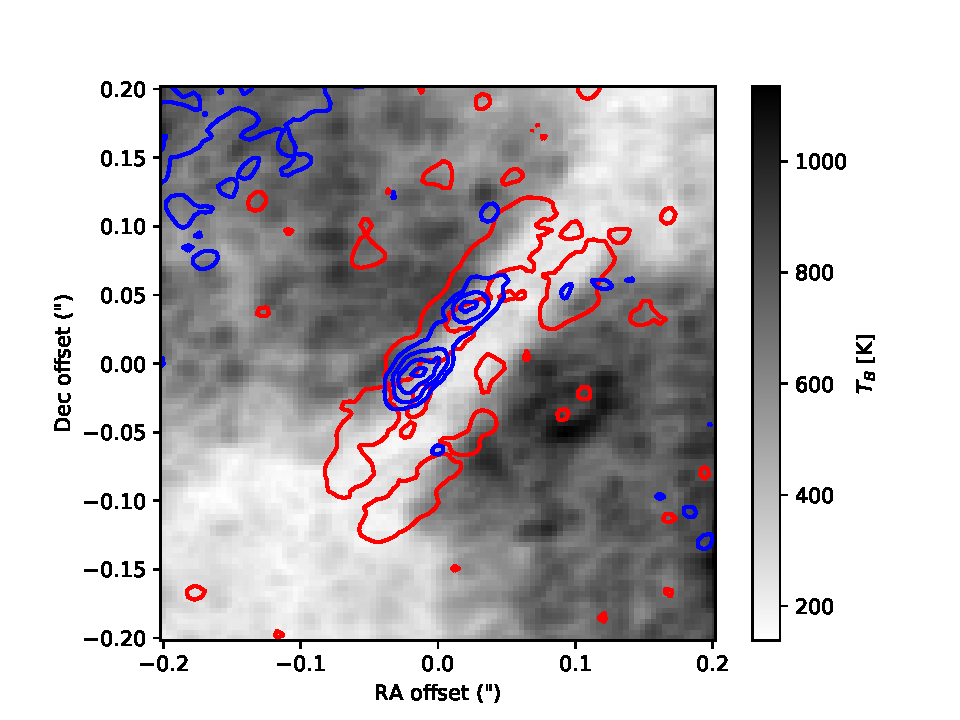
\includegraphics[scale=1,width=4in]{figures/SiO_8-7_on_NaClv=2_26-25.pdf}
\caption{Peak intensity map of SiO v=0 J=8-7 (gray scale), NaCl v=2 J=26-25
(red contour; 200 K) and {SiO v=5 J=8-7} (blue contours; 300, 400, 500, and 600
K).  The blue contours in the upper-left come from a blend with a different
line.
}
\label{fig:sioonnacl}
\end{figure*}


While the most prominent spectral features were the SiO and \water lines that
have previously been observed \cite{Goddi2013a,Hirota2014a}, there were dozens
of lines that remained unidentified in our initial study \cite{Ginsburg2018b}.
We have now identified these lines as transitions of NaCl and KCl, noting the
excellent correspondence between the observed and measured/catalogued
frequencies \cite{Caris2002a,Caris2004a,Muller2005a,Lovas2005b,Pickett1998a}.
We additionally searched databases of transitions of these same species with
more quanta of vibrational excitation, and found additional matches
\cite{Barton2014a,Cabezas2016a}, with confident detections up to as much as
$v=6$.

%AG: the v=7 detections are <5-sigma; they're probably real, but not confident.

The emission from these lines comes
from a narrow range in both position and velocity.  By fitting thin Keplerian
disk models to the position-velocity diagrams of the lines, we constrain the
emission region to be 30-60 AU from the central source.  The observed emission
peaks at $\pm13$ AU above and below the midplane of the continuum disk, which
may be either a physical height or an effect of obscuration by the optically
thick continuum.  The emission does not extend beyond this height, indicating
that, unlike SiO and \water, the salts do not trace the outflow.

%BAM: We aren't allowed to tell the reader how to feel (in Science).  Meaning,
%we can't say something is 'surprising.'  That's up to the reader to decide.
%no "we were shocked to see shocks"?  Boo.

Once in the gas phase, however, we expect salts to rapidly deplete back into
dust grains \cite{Cherchneff2012a}.  Since we observe them in emission, with
narrow velocity line profiles, they must be released into the gas phase either
by grain destruction by chemical production from simple gas-phase
precursors, likely elemental atomic gas (either neutral or ionized Na and K).
Because previous studies have %ruled out the presence of 
failed to detect any atomic
recombination lines (from atomic ions recombining with electrons) in this
source
% rlp: note that Na and K MUST be ionized in the > 1000 K gas near the 
% central source; the electrons released from Na and K are presumably the
% source of the low frequency (< 43 GHz) continuum emission from SrcI
% via the H- free-free emission (electron-neutral brehmsstrahlung)
%
% and therefore demonstrated that there is no ionized gas around Source I
\cite{Plambeck2016a,Baez-Rubio2018a}, we reject the atomic formation route. We
therefore suggest that the salts are produced by dust destruction, either
via sputtering by high-energy particles \cite{Schilke1997a} or by thermal
desorption of the outer dust layers \cite{Decin2016a}.  The SiO emission seen
in the outflow confirms that dust destruction is occurring as part of the outflow
launch process.

%Since we see SiO tracing
%the outflow, and SiO is also released by grain destruction, we infer that...
%The small scale
%height of the observed salt emission therefore implies that grain destruction
%is an efficient and rapid process in disk-launched winds.

%Again, we can present our viewpoint based on the data, but it's up to the
%reader to decide if that is what 'must' be happening.

The detection of highly vibrationally excited transitions of these species,
with upper-state energy levels of as much as $\sim$3000~K, is suggestive of
extreme physical or radiative conditions.
%The vibrationally excited transitions observed suggest that radiative
%excitation is important in this environment.
The molecular transitions we
observe have high Einstein A values, in the range $\sim10^{-3}-10^0$ s$^{-1}$, and
correspondingly high critical densities $n_{cr} \sim10^{8}$ \percc for v=0 and
$n_{cr} \sim 10^{12}$ for $v>=1$ {\bf [rlp: I thought the RADEX plots showed
$10^{11}$ for the vibrational levels; in any case, seems weird that 3 orders
of magnitude in A give 4 orders of magnitude in critical density]}, 
where $v$ is the vibrational quantum number.
Collisional excitation alone cannot explain the different vibrational states
being observed at a similar brightness level. The rovibrational $\Delta v=1$
transitions of NaCl and KCl occur in the 25-35 \um and 35-45 \um range,
respectively.  Since a blackbody with $T\sim100$ K peaks at $\lambda\sim30$
\um, and the observed disk brightness temperature is around 100-300 K at the
radii where salts are observed, it is plausible that strong radiation from the
disk in the mid-infrared is responsible for exciting the molecules.  However,
we have not been able to assemble a self-consistent model explaining both the
rotational and vibrational excitation ladders of NaCl or KCl.  In the
supplemental material, we describe  and evaluate several possible
excitation mechanisms that are less likely but not ruled out.

\begin{figure}
    \begin{tabular}{lr}
    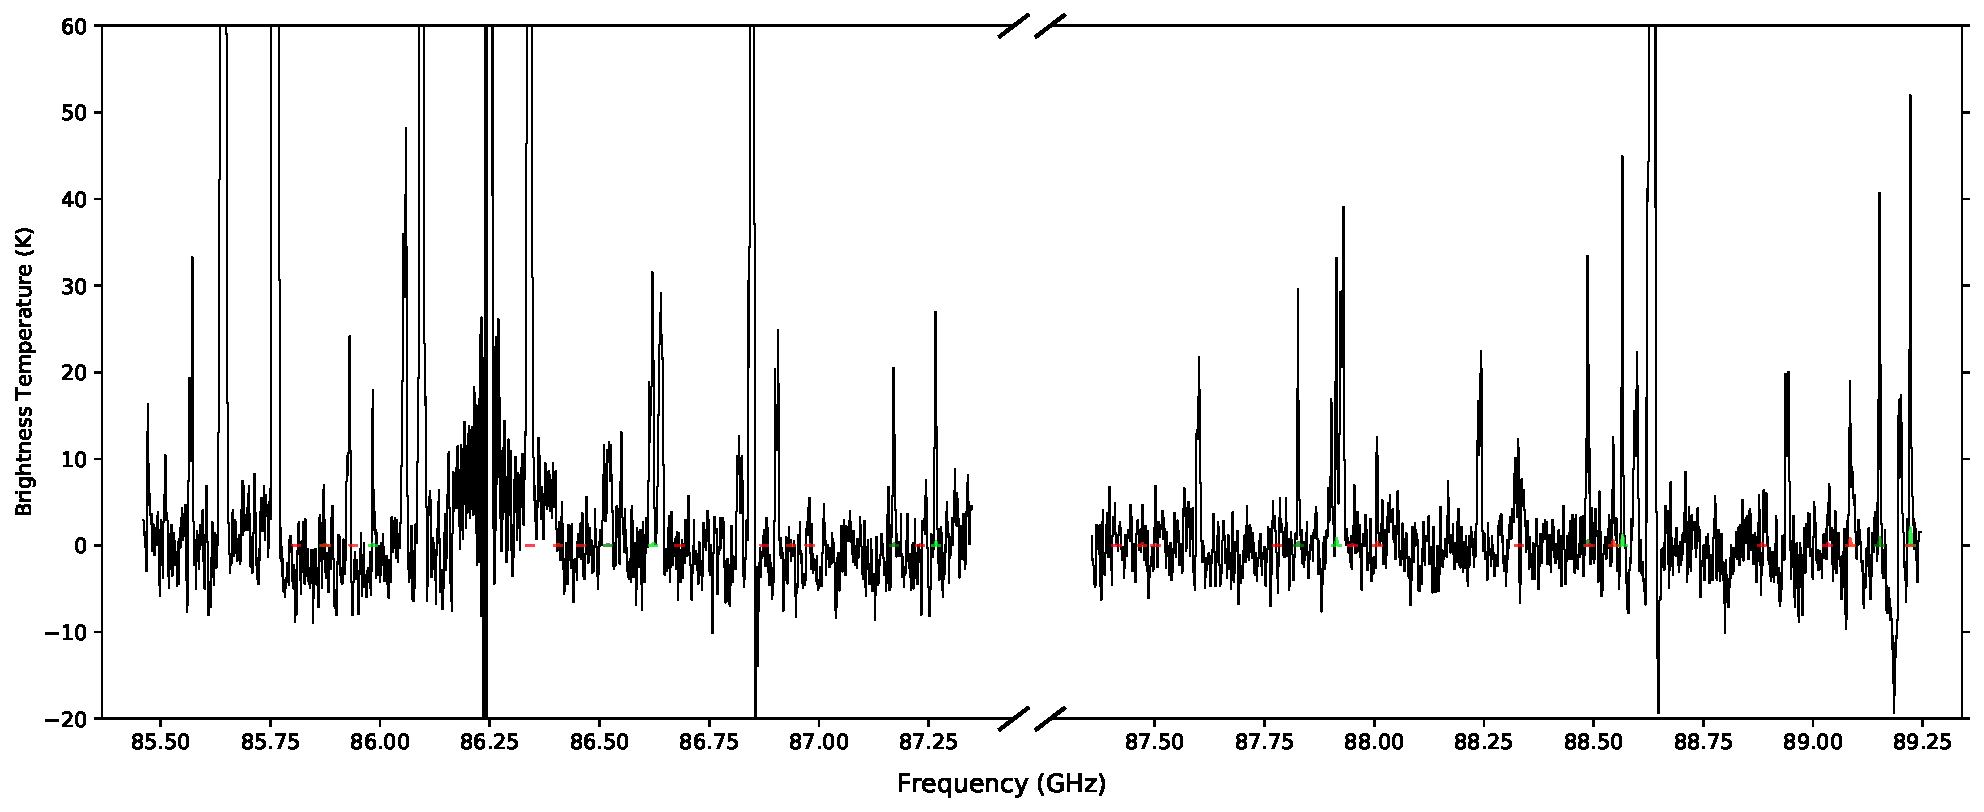
\includegraphics[scale=1,width=3.0in]{{figures/squash_lte_overlay_K_a_OrionSourceI_B3_spw1_robust0.5}.pdf}&
    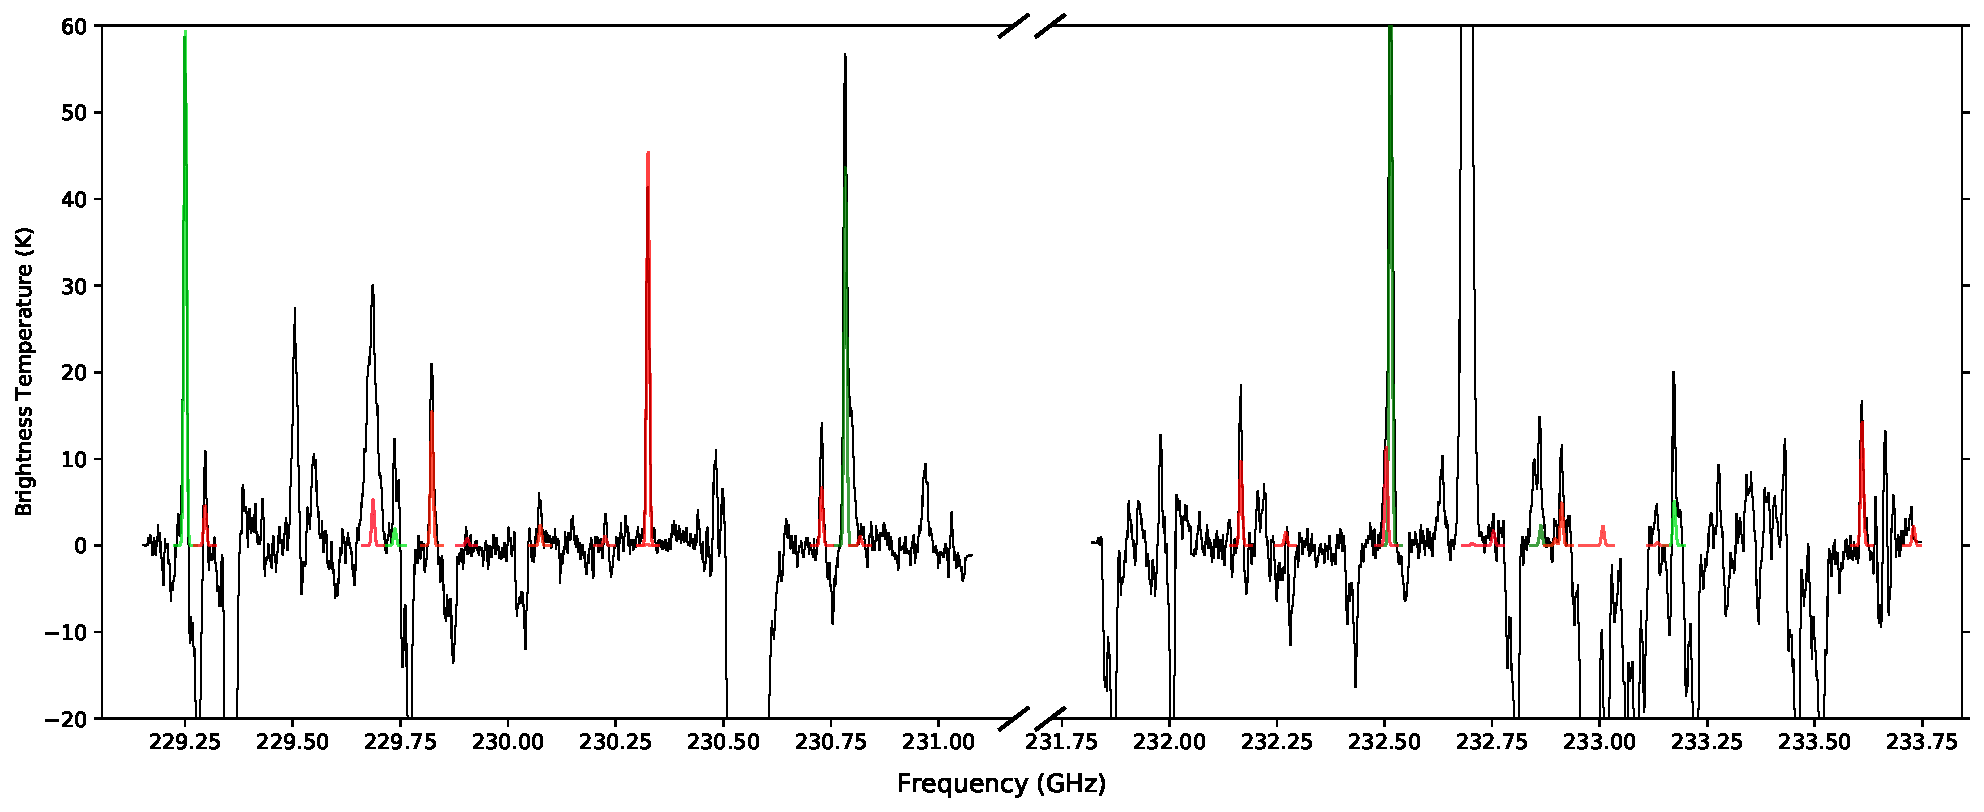
\includegraphics[scale=1,width=3.0in]{{figures/squash_lte_overlay_K_a_OrionSourceI_B6_spw1_robust0.5}.pdf}\\
    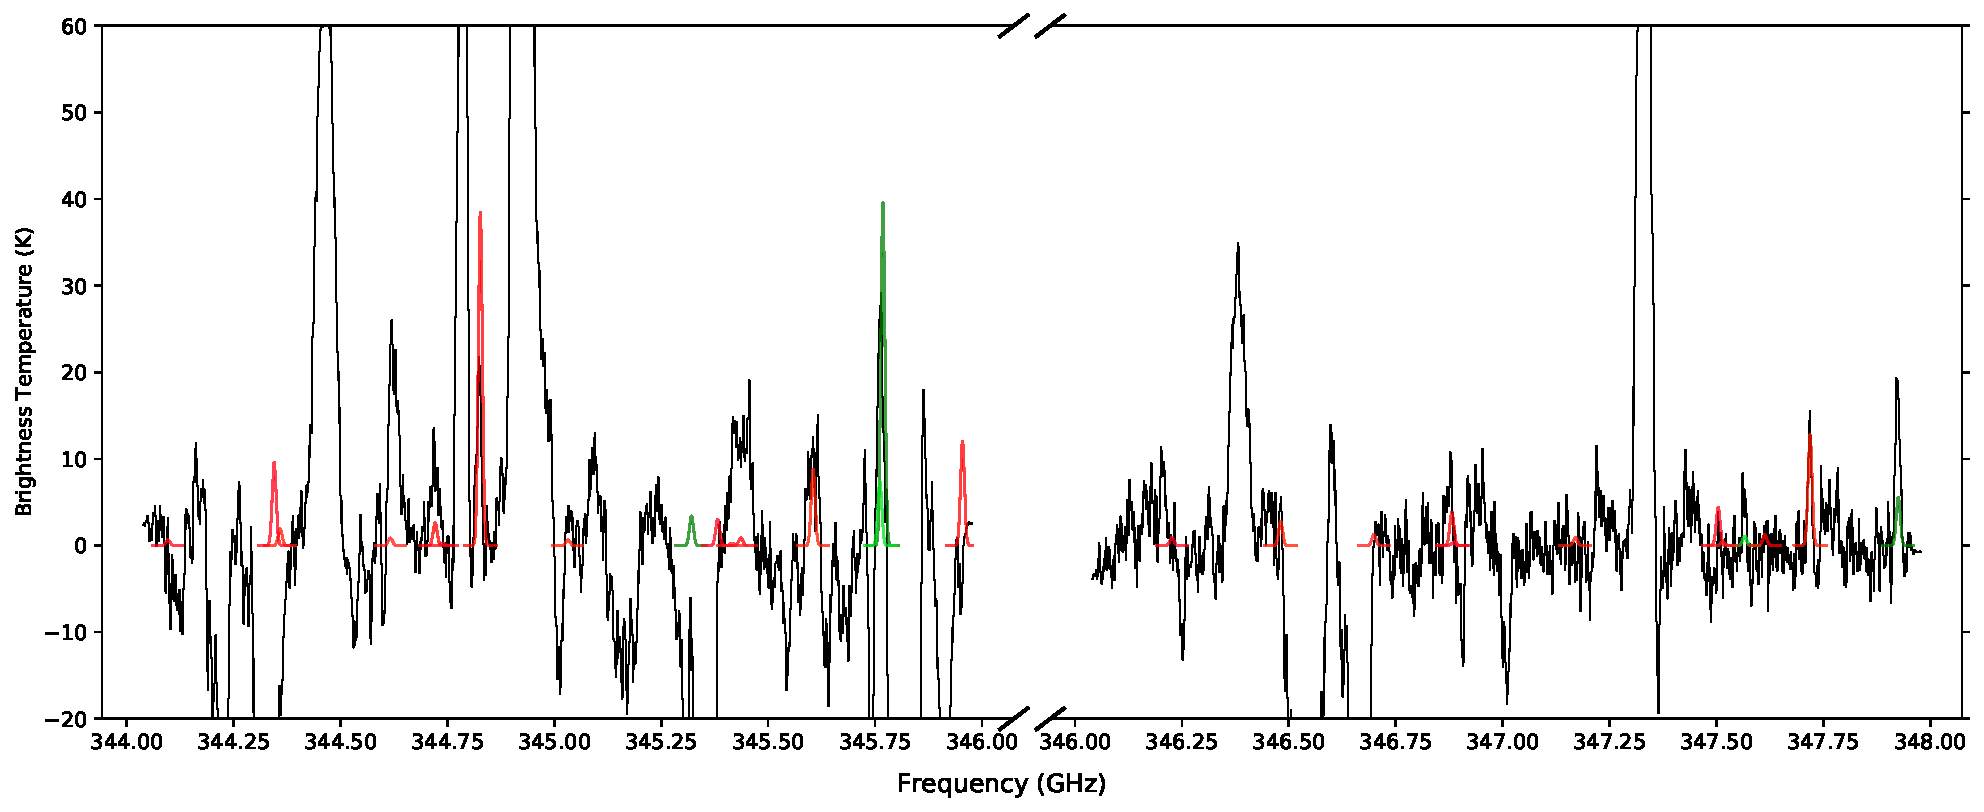
\includegraphics[scale=1,width=3.0in]{{figures/squash_lte_overlay_K_a_OrionSourceI_B7.lb_spw1_robust0.5}.pdf}&
    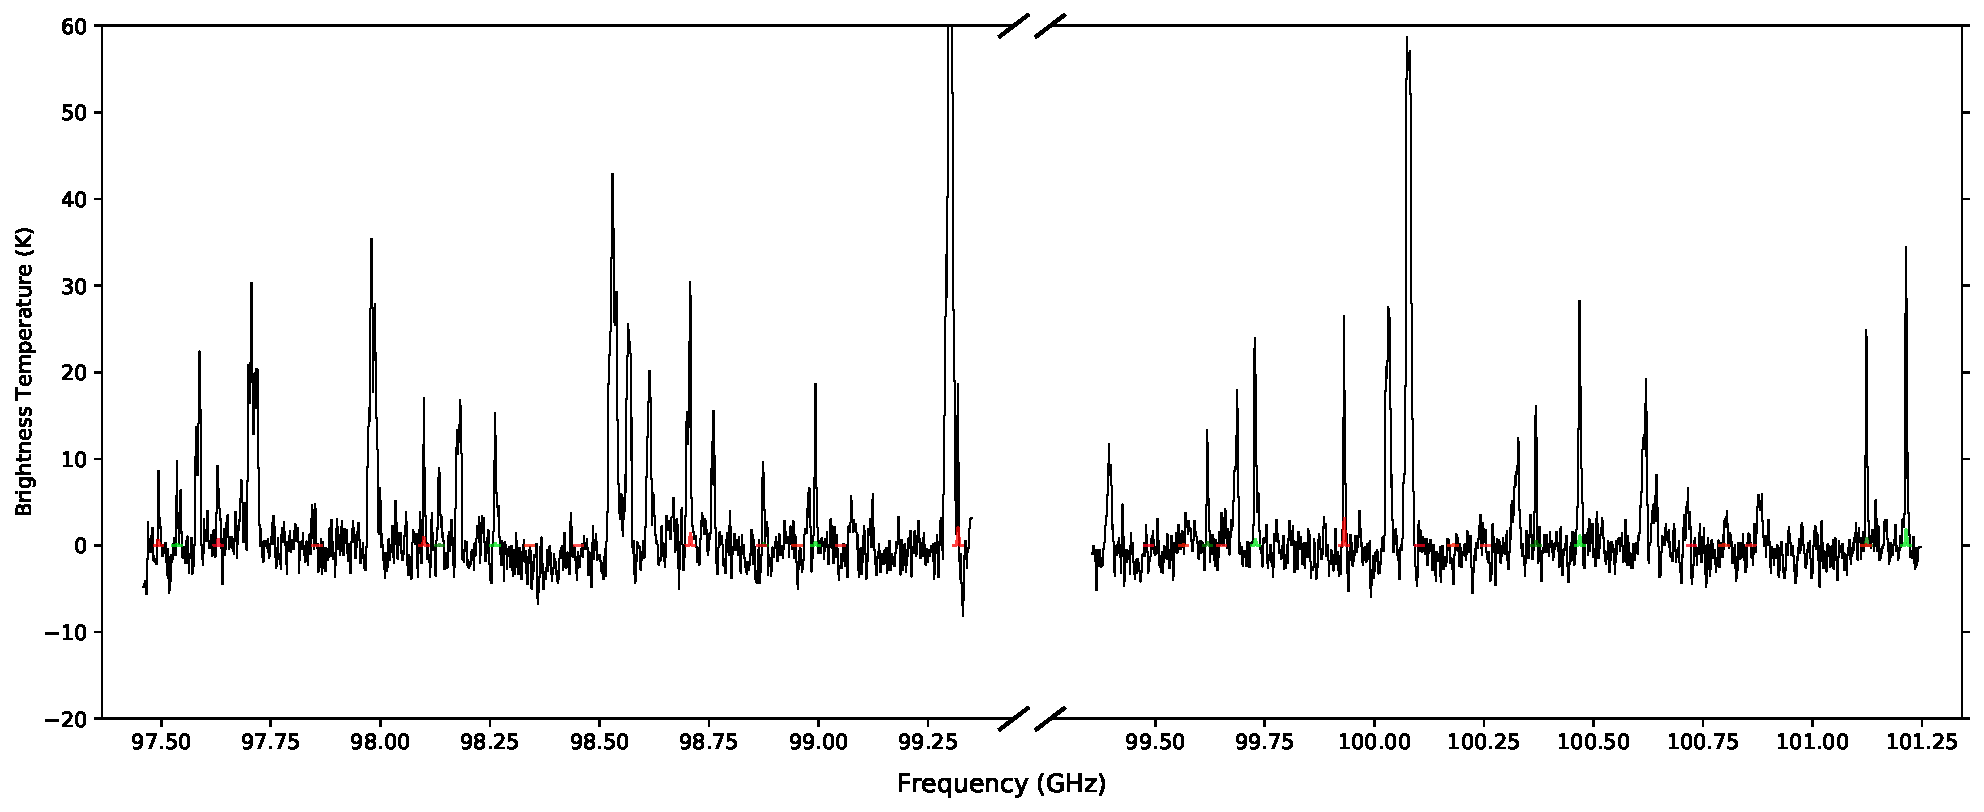
\includegraphics[scale=1,width=3.0in]{{figures/squash_lte_overlay_K_b_OrionSourceI_B3_spw3_robust0.5}.pdf}\\
    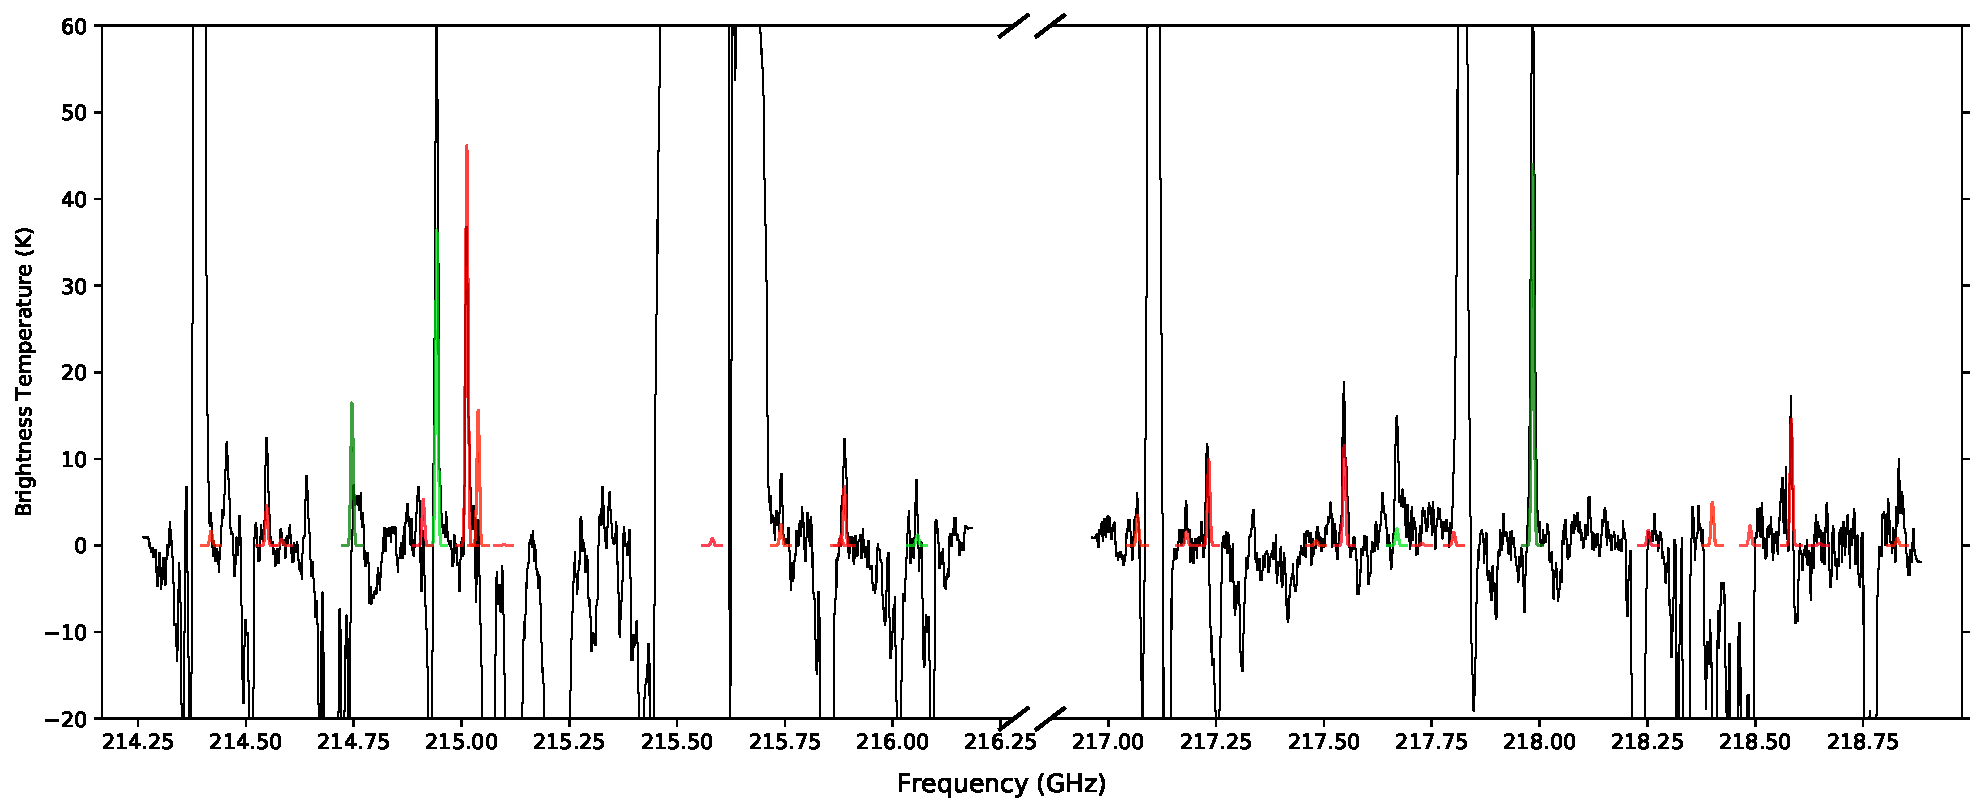
\includegraphics[scale=1,width=3.0in]{{figures/squash_lte_overlay_K_b_OrionSourceI_B6_spw3_robust0.5}.pdf}&
    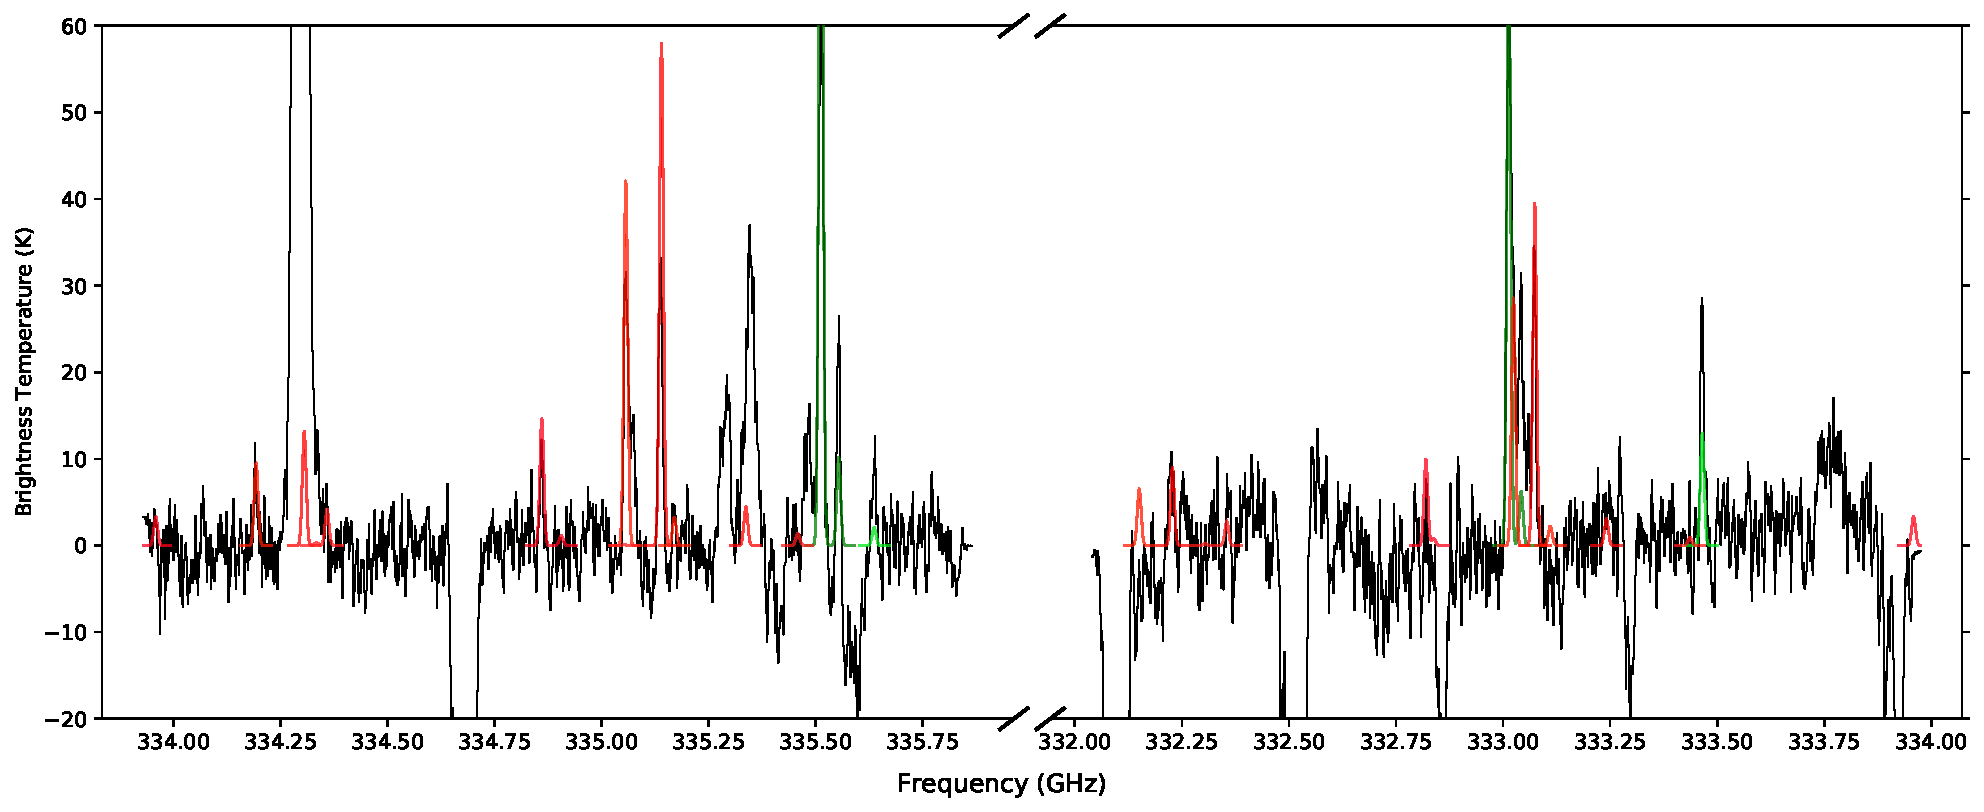
\includegraphics[scale=1,width=3.0in]{{figures/squash_lte_overlay_K_b_OrionSourceI_B7.lb_spw3_robust0.5}.pdf}\\
    \end{tabular}
    \label{fig:spectra}
    \caption{Spectra with NaCl (green) and KCl (red) models overlaid.
    The models assume a constant, single excitation temperature $T_{ex}=1000$ K
    and column densities $N(\mathrm{NaCl})=4\ee{12}$ \persc and $N(\mathrm{KCl})=2\ee{12}$ \persc.
    The $^{37}$Cl isotopologues are included at half those column densities,
    and the $^{41}$K isotopologue at one quarter.
    These models are not a good fit to the data, underpredicting the vibrationally
    excited level populations, but they highlight that the lines with expected
    emission are uniformly strongly detected.
    }
\end{figure}


% The detection of NaCl and KCl in our current dataset was serendipitous.  As a
% result, the observations were not optimized for unraveling the physical and
% chemical conditions underlying their presence and excitation, hindering our
% ability to obtain a full picture of the exact utility of these salts as
% tracers.  Nevertheless, we obtain several important conclusions from these
% detections.

We conclude that these newly detected transitions uniquely trace the disk
around a massive protostar.  Since they appear to be an unambiguous tracer of
high-mass protostellar disks, if they behave the same in other high-mass disks,
they will facilitate kinematic measurements of disks and therefore direct mass
measurements of the contained stars.  Access to such a tool would finally make
direct comparisons between high- and low-mass star formation possible.

Since these molecules contain atoms usually trapped in dust and therefore
rarely seen in the molecular ISM, they may serve as a tool for directly
measuring absolute metallicity in an environment that is typically far too
chemically complex and obscured for other methods to work.  Since these
species are released into the ISM only by supernovae, these transitions
could prove a powerful probe of supernova feedback in high-extinction
regions. % this is pretty far-fetched...

% Of these species,
% Na is produced only in massive star supernovae, while K and Cl are produced in
% white dwarf supernovae  <-- I don't know if this is true.  cosmic-origins.org +
% wikipedia say so, but those are loose.  Arnett '96 doesn't seem to have a table
% of "this comes from here".

%This last paragraph should probably be two or three instead of one?  Note that
%we explicitly cannot include any 'forward-looking' projects that *we plan*
%(meaning, we cannot say that follow-up studies will look at X or Y).  We can
%speculate a bit (it's a fine line) on what these lines might be useful for in
%a general sense, however.


\bibliographystyle{Science}
\bibliography{extracted}

% Following is a new environment, {scilastnote}, that's defined in the
% preamble and that allows authors to add a reference at the end of the
% list that's not signaled in the text; such references are used in
% *Science* for acknowledgments of funding, help, etc.

\begin{scilastnote}
\item[] \textbf{Supplementary Materials}

\vspace{-1em}
www.sciencemag.org

\vspace{-1em}
Materials and Methods

\vspace{-1em}
Figures S1, S2

\vspace{-1em}
Tables S1, S2, S3, S4, S5

\vspace{-1em}
References (39-56)

\item[] \textbf{Acknowledgements}
\item[] 
The National Radio Astronomy Observatory is a facility of the National Science
Foundation operated under cooperative agreement by Associated Universities,
Inc. The Green Bank Observatory is a facility of the National Science
Foundation operated under cooperative agreement by Associated Universities,
Inc. Support for B.A.M. was provided by NASA through Hubble Fellowship grant
\#HST-HF2-51396 awarded by the Space Telescope Science Institute, which is
operated by the Association of Universities for Research in Astronomy, Inc.,
for NASA, under contract NAS5-26555. 
This paper makes use of the following ALMA data: ADS/JAO.ALMA\#2016.1.00165.S
ALMA is a partnership of ESO (representing its member states), NSF (USA) and
NINS (Japan), together with NRC (Canada), MOST and ASIAA (Taiwan), and KASI
(Republic of Korea), in cooperation with the Republic of Chile. The Joint ALMA
Observatory is operated by ESO, AUI/NRAO and NAOJ.



\clearpage

Supplementary Materials for


\title{Orion \sourcei's disk is salty}

\author{
Adam Ginsburg\\
\nraojansky\\
e-mail: aginsbur@nrao.edu; adam.g.ginsburg@gmail.com\\
Brett McGuire\\
\hubble\\
\nraocv\\
\cfa\\
John Bally\\
\casa\\
Ciriaco Goddi\\
\allegro\\
\radboud\\
Richard Plambeck\\
\berkeley\\
Melvyn Wright\\
\berkeley\\
}



\item[] \textbf{This PDF file includes:}

%\vspace{-1em}
%www.sciencemag.org

\vspace{-1em}
Materials and Methods

\vspace{-1em}
Figures S1, S2

\vspace{-1em}
Tables S1, S2, S3, S4, S5

\vspace{-1em}
References (39-56)

 \end{scilastnote}
 
 \clearpage
 
 \part*{Materials \& Methods}

\renewcommand{\thefigure}{S\arabic{figure}}
\renewcommand{\thetable}{S\arabic{table}}
\renewcommand{\theequation}{S\arabic{equation}}
\setcounter{figure}{0}
\setcounter{table}{0}
\setcounter{equation}{0}


\section*{Observations}

The observations presented here are described in \cite{Ginsburg2018b} as part
of ALMA project 2016.1.00165.S.  We use the robust 0.5 weighted spectral cubes
from all three bands (B3 3 mm, B6 1 mm, B7 0.85 mm) for our spectroscopic analysis.

Appendix D of that paper describes the spectral extraction method,
which we summarize here.  We used the U232.511 line (which we now identify as
NaCl v=1 J=18-17) to find the velocity centroid for each (spatial) pixel
across the \sourcei disk.  We shifted the spectrum along
each such pixel to 0 \kms, then averaged the shifted spectra over the region with
significant emission in the NaCl line.  
The
averaging area is approximately the extent of the continuum disk, 0.03 square
arcseconds, or about 4, 20, and 40  beam areas, resulting
in an improvement in the signal-to-noise of about $2\times$, $4\times$, and $6\times$
respectively in Band 3, 6, and 7.
This stacked spectrum, shown in Figures \ref{fig:spectrab3}-\ref{fig:spectrab7},
% is the average spectrum across the disk identified in \citet{Ginsburg2018b}: it
traces material just above and below the optically thick continuum disk
(Figure \ref{fig:spatial}), and for the lines discussed here, includes no
emission associated with the outflow.  
% OK, I'm putting my preferred sentence here for now. It could be moved
% to a footnote or the figure caption if desired. - Dick
% AG: I don't like this because it sounds like the lines are narrower than we
% observe, which isn't right: they are narrower than what you get by averaging
% over the observations, but they are wider than you get by pointing a single
% beam at the disk as is.
Because this procedure removes the rotational velocity field of the disk,
lines in the stacked spectrum are narrower than one would observe in
a lower spatial resolution observation of the disk.  One may think of the
stacked spectrum as the output of a matched filter that is optimized for
detection of disk emission.

% The stacked spectrum is equivalent to that
% obtained with a matched filter using a narrow (delta-function) filter at each
% position tuned to the appropriate centroid velocity.

% We have clearly identified the carrier of the majority of unidentified lines in
% the \citet{Ginsburg2018b} spectra (only 2-3 lines are unidentified in the B6/B7
% spectra, though there are several in B3 we have not identified).

In the appendix of \cite{Ginsburg2018b}, we listed over 20 unidentified 
lines in the B6 ALMA spectra, and commented that ``there is no
consistent pattern to the detected lines and no individual species can explain
more than a few of the observed lines.''  This statement was incorrect, as
there are obvious carriers for the majority of the unidentified lines that we
had simply overlooked: NaCl, KCl, and their isotopologues.  The
detected lines have amplitudes in the range 0.5-3 mJy beam$^{-1}$, corresponding
to brightness temperatures 5-20 K.  

In Figures \ref{fig:spectrab3}-\ref{fig:spectrab7}, we have labeled all of the
detections and marginal detections of salt lines, as well as the most prominent
outflow (e.g., SiO and H$_2$O) lines.  Only 2-3 emission lines are now
unidentified in the B6 and B7 spectra, though there are over a dozen in B3 that
we have not identified. 

We also tentatively identify broad lines at 229.7 GHz and 334.4 GHz as AlO.  
{\bf: [rlp: I see nothing in the spectrum at 334.4 GHz; I question whether
we should mention AlO at all.]} If
the identification is correct, these lines are broad because of the rich hyperfine
spectrum of AlO.

% I count 15 unidentified emission lines in B3; I added "emission" above 
% because there are lots of unidentified absorption lines from foreground gas. - Dick
%
%We additionally labeled
%\emph{some} of the lines that were not detected because of severe confusion

\begin{figure*}[!htp]
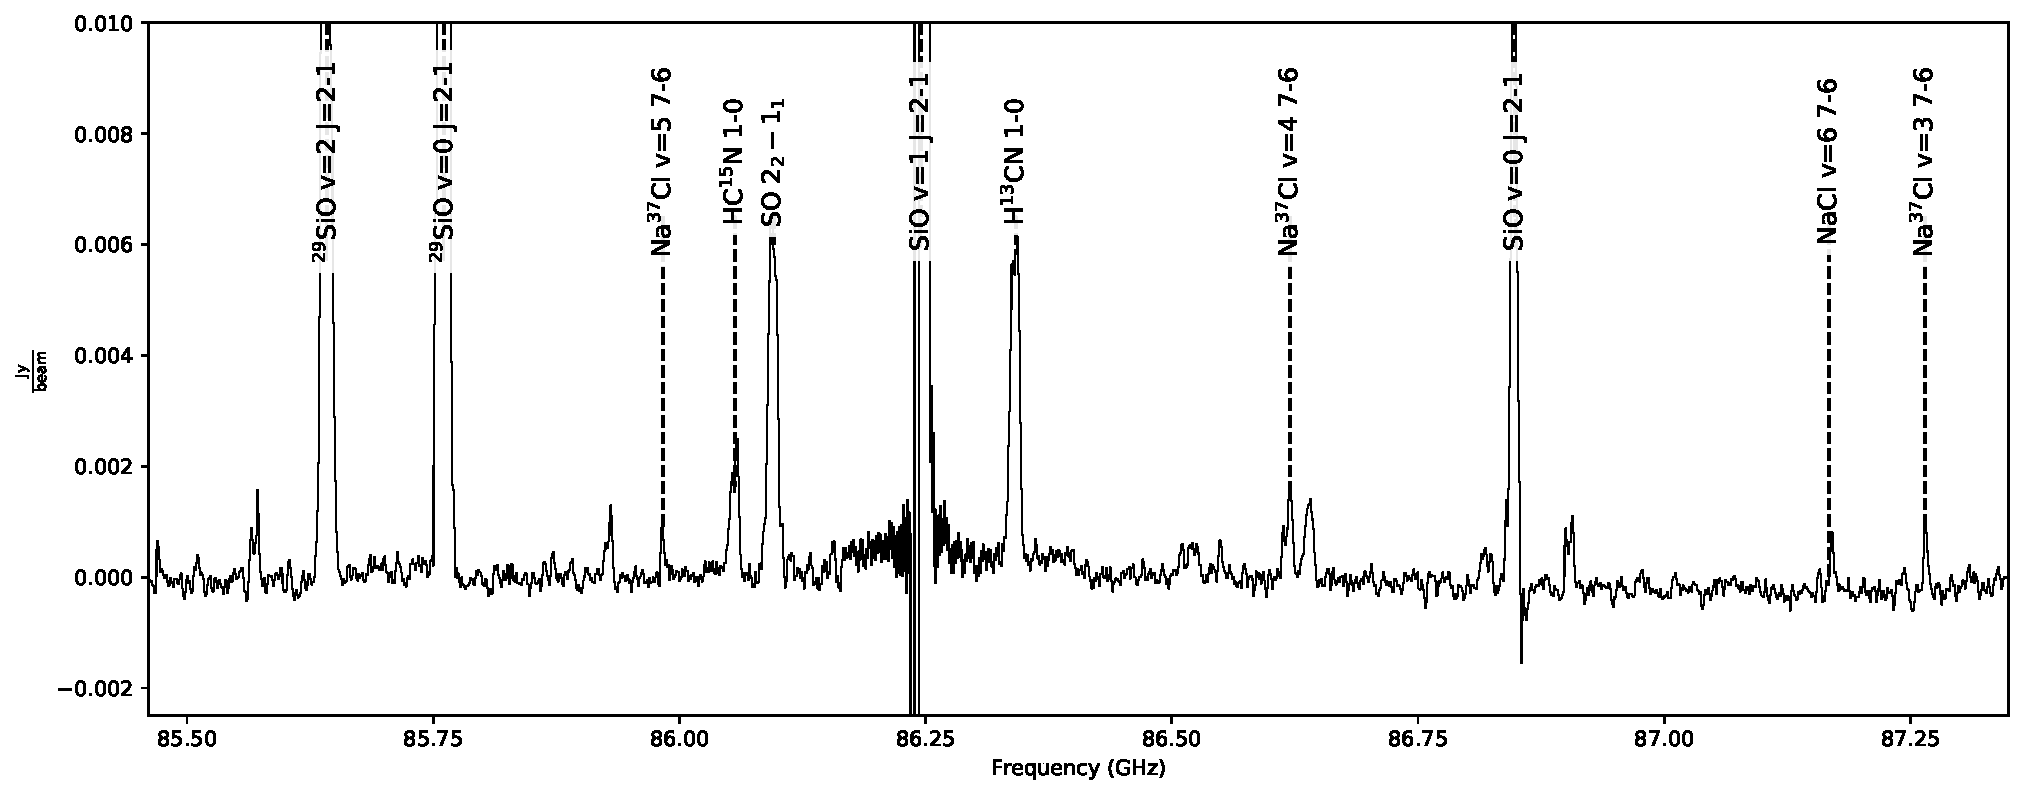
\includegraphics[scale=1,width=5.5in]{{figures/lines_labeled_OrionSourceI_B3_spw0_robust0.5}.pdf}
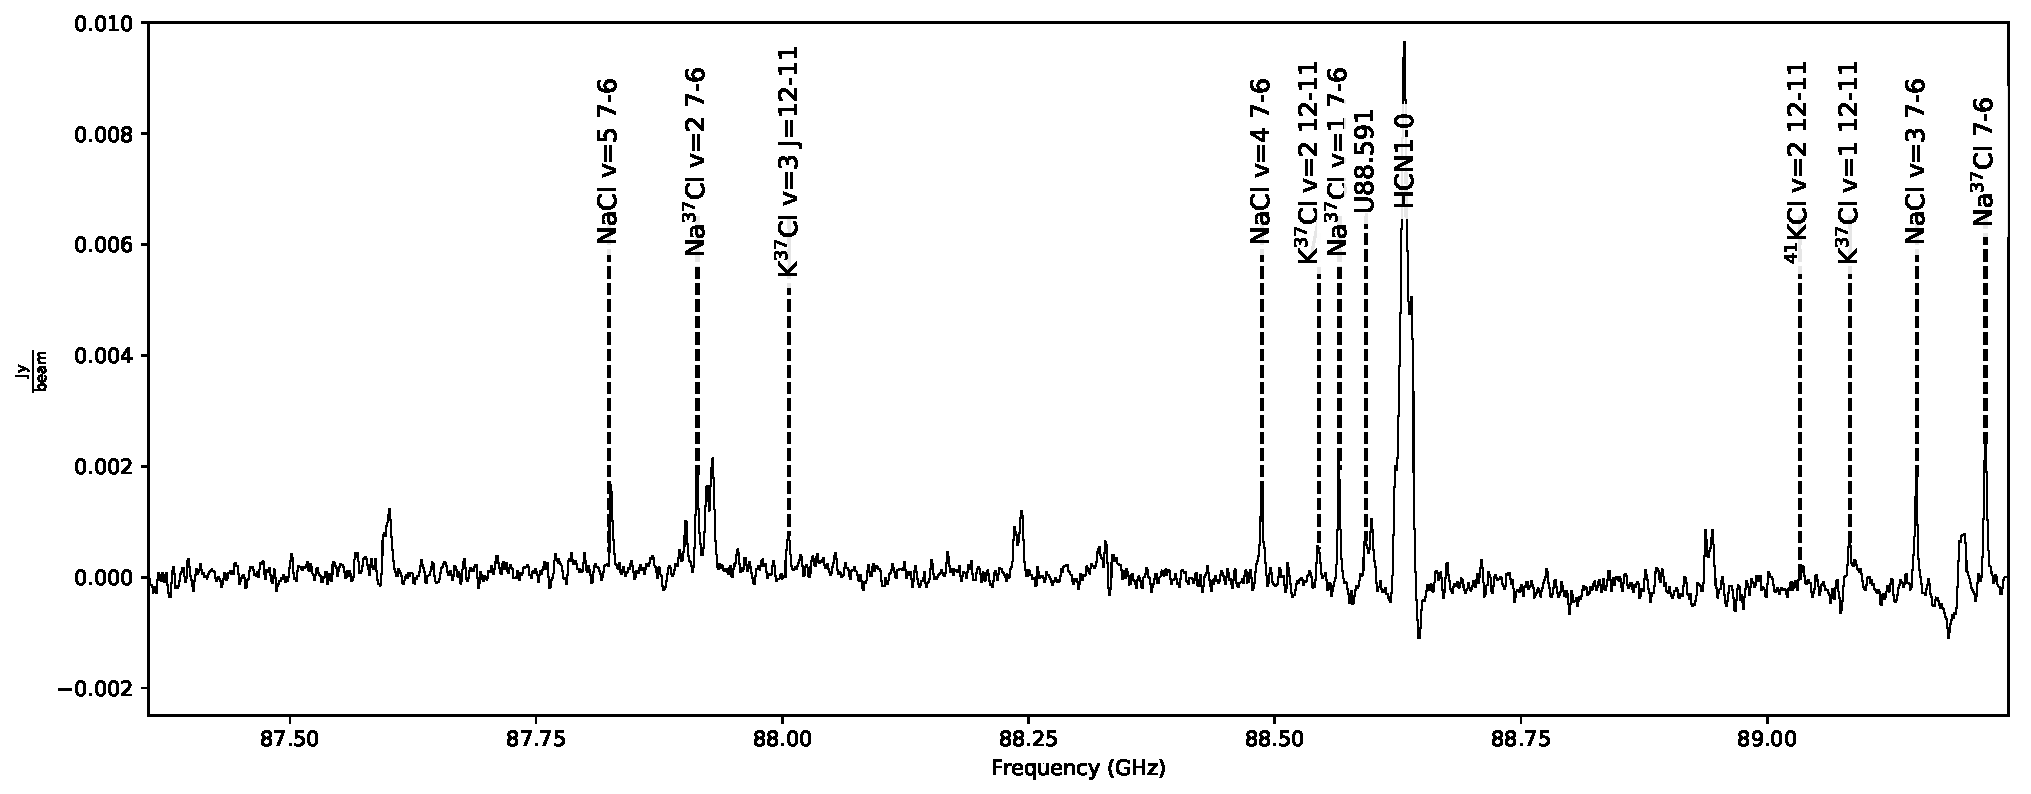
\includegraphics[scale=1,width=5.5in]{{figures/lines_labeled_OrionSourceI_B3_spw1_robust0.5}.pdf}
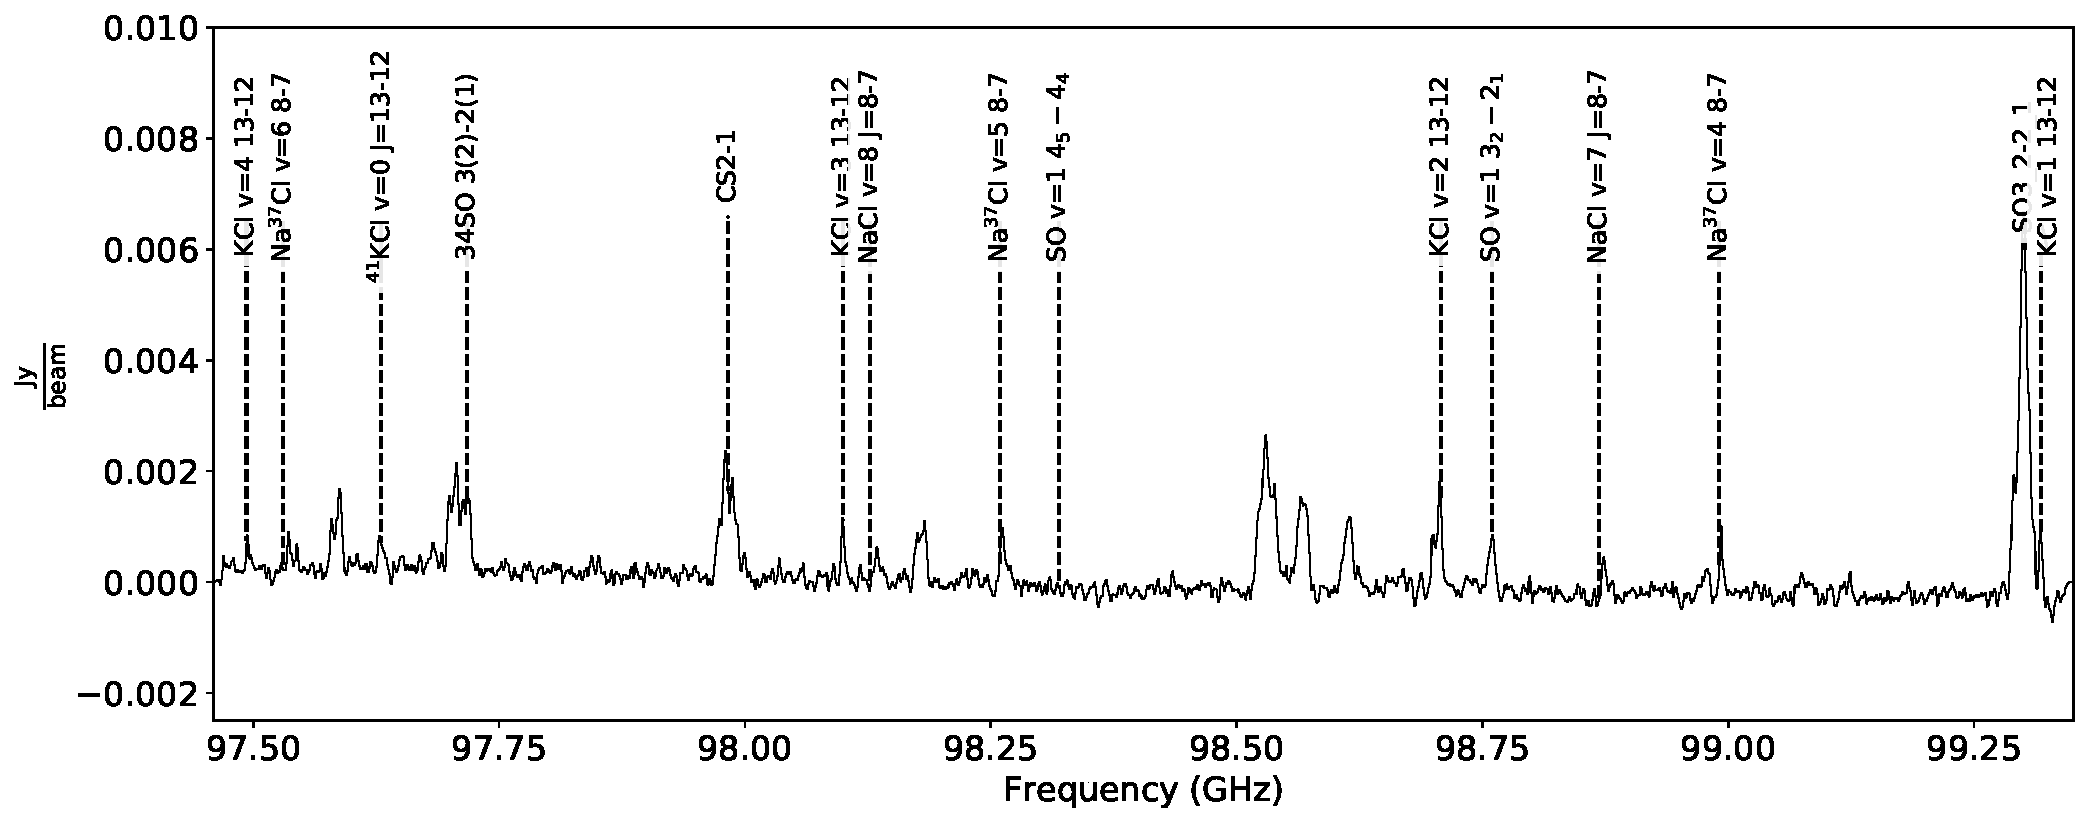
\includegraphics[scale=1,width=5.5in]{{figures/lines_labeled_OrionSourceI_B3_spw2_robust0.5}.pdf}
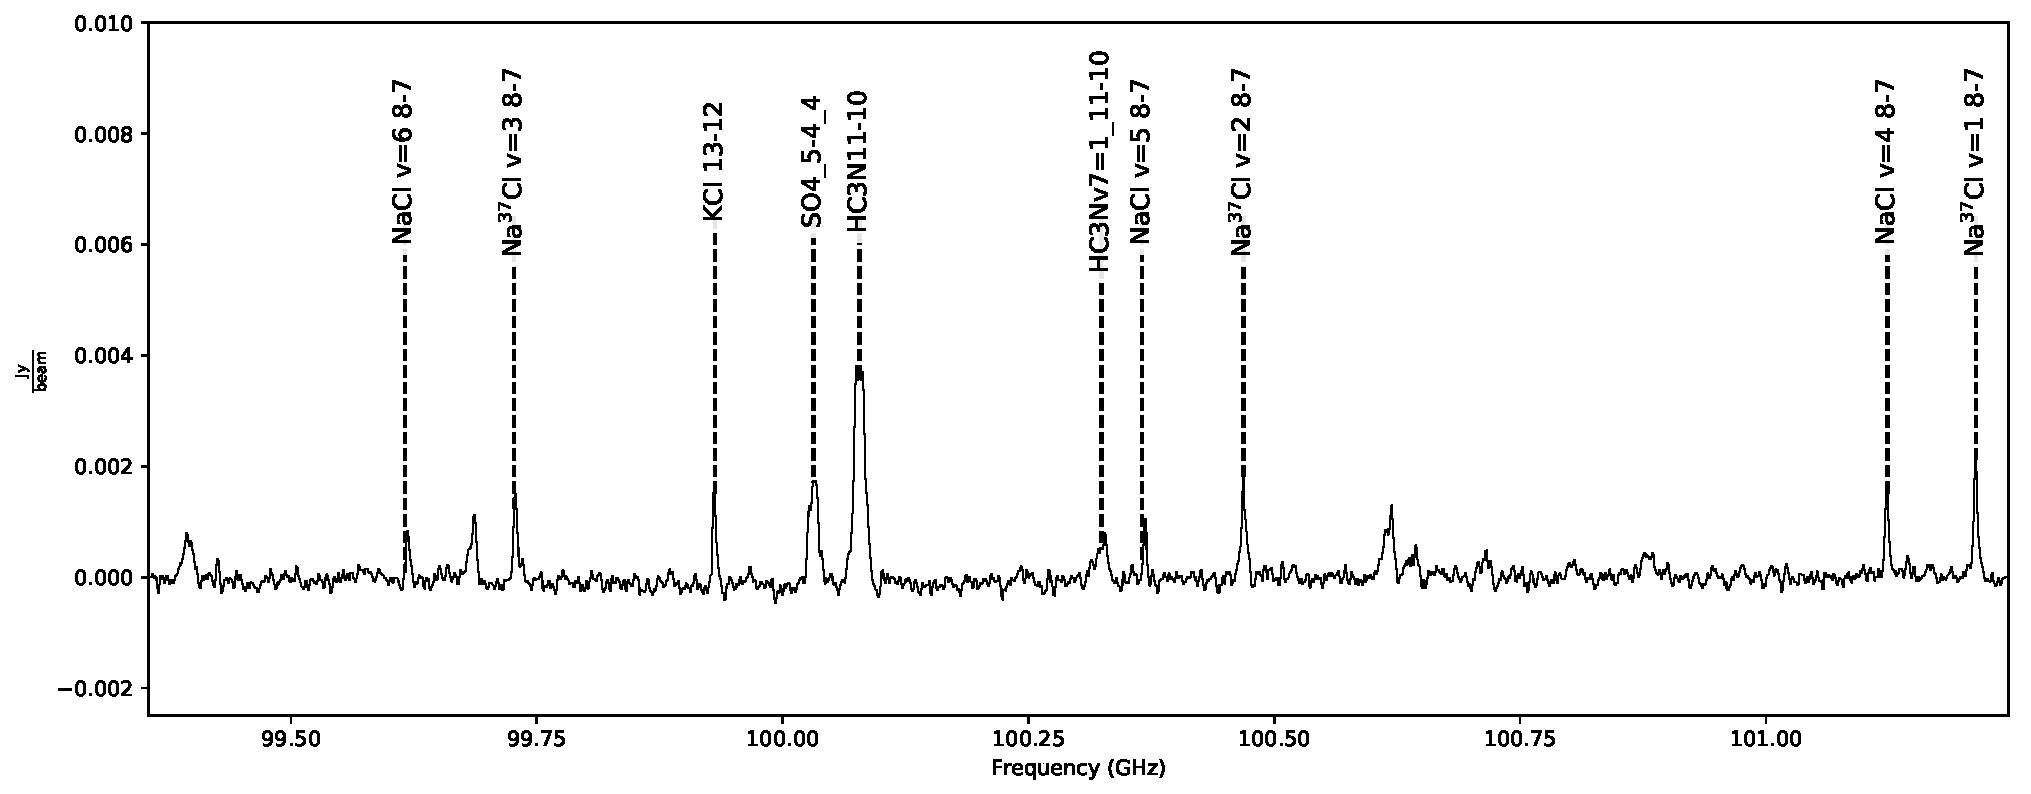
\includegraphics[scale=1,width=5.5in]{{figures/lines_labeled_OrionSourceI_B3_spw3_robust0.5}.pdf}
\caption{Stacked spectra  B3}
\label{fig:spectrab3}
\end{figure*}
\begin{figure*}[!htp]
    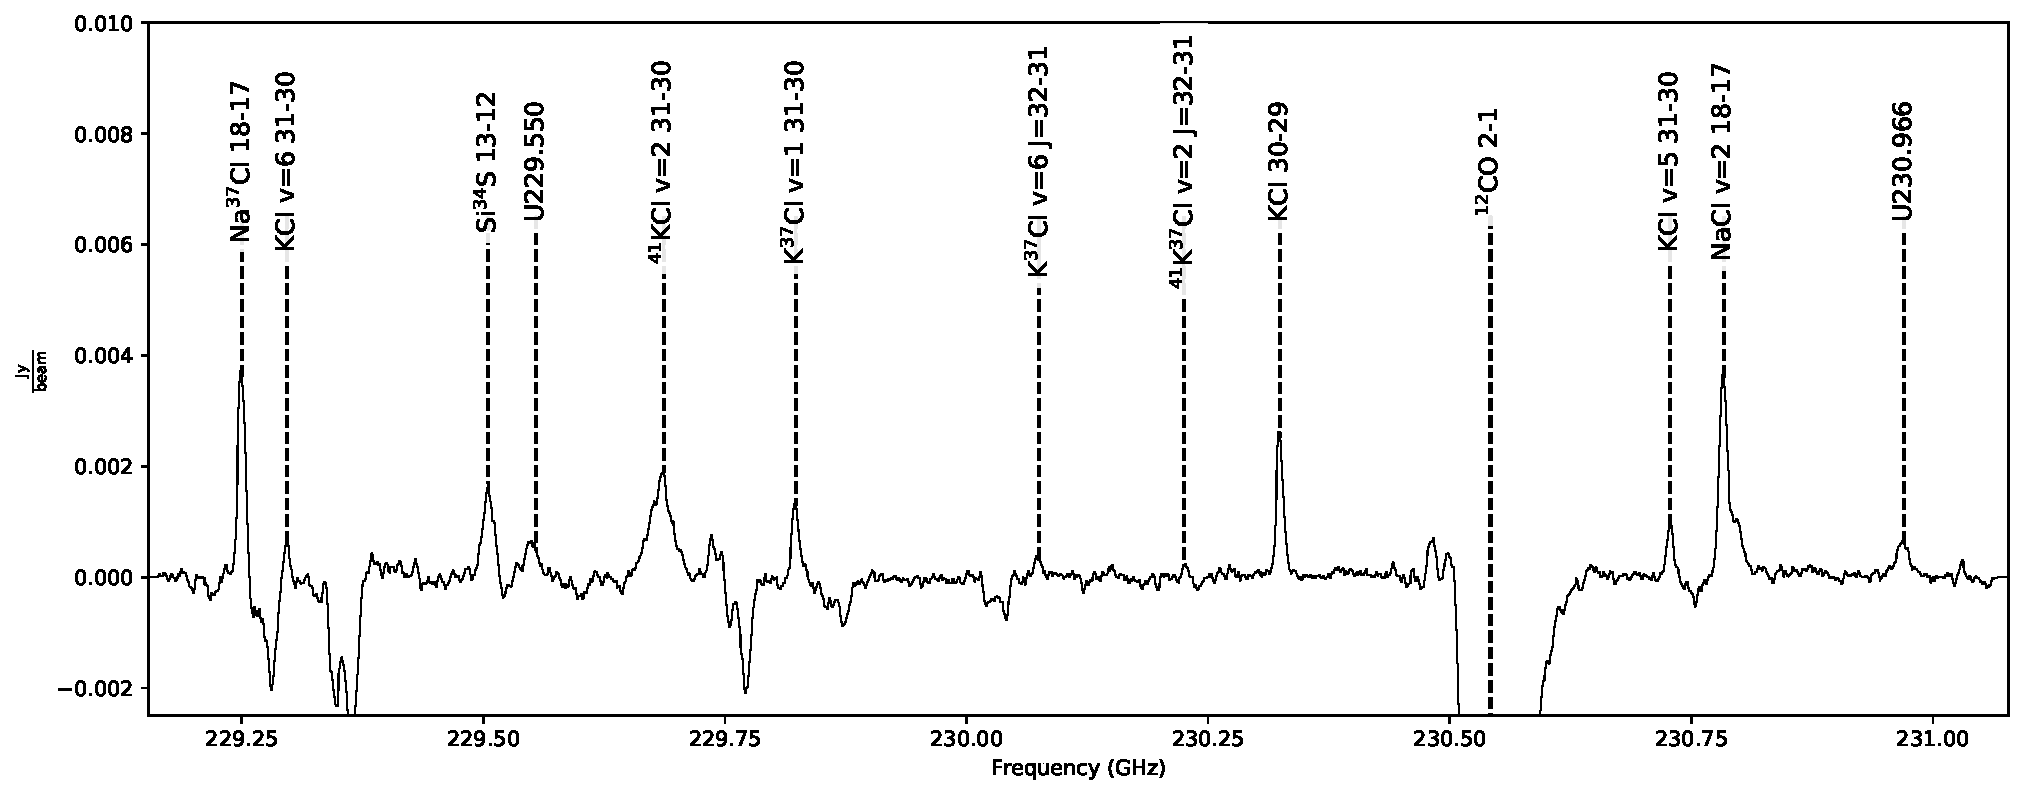
\includegraphics[scale=1,width=5.5in]{{figures/lines_labeled_OrionSourceI_B6_spw0_robust0.5}.pdf}
    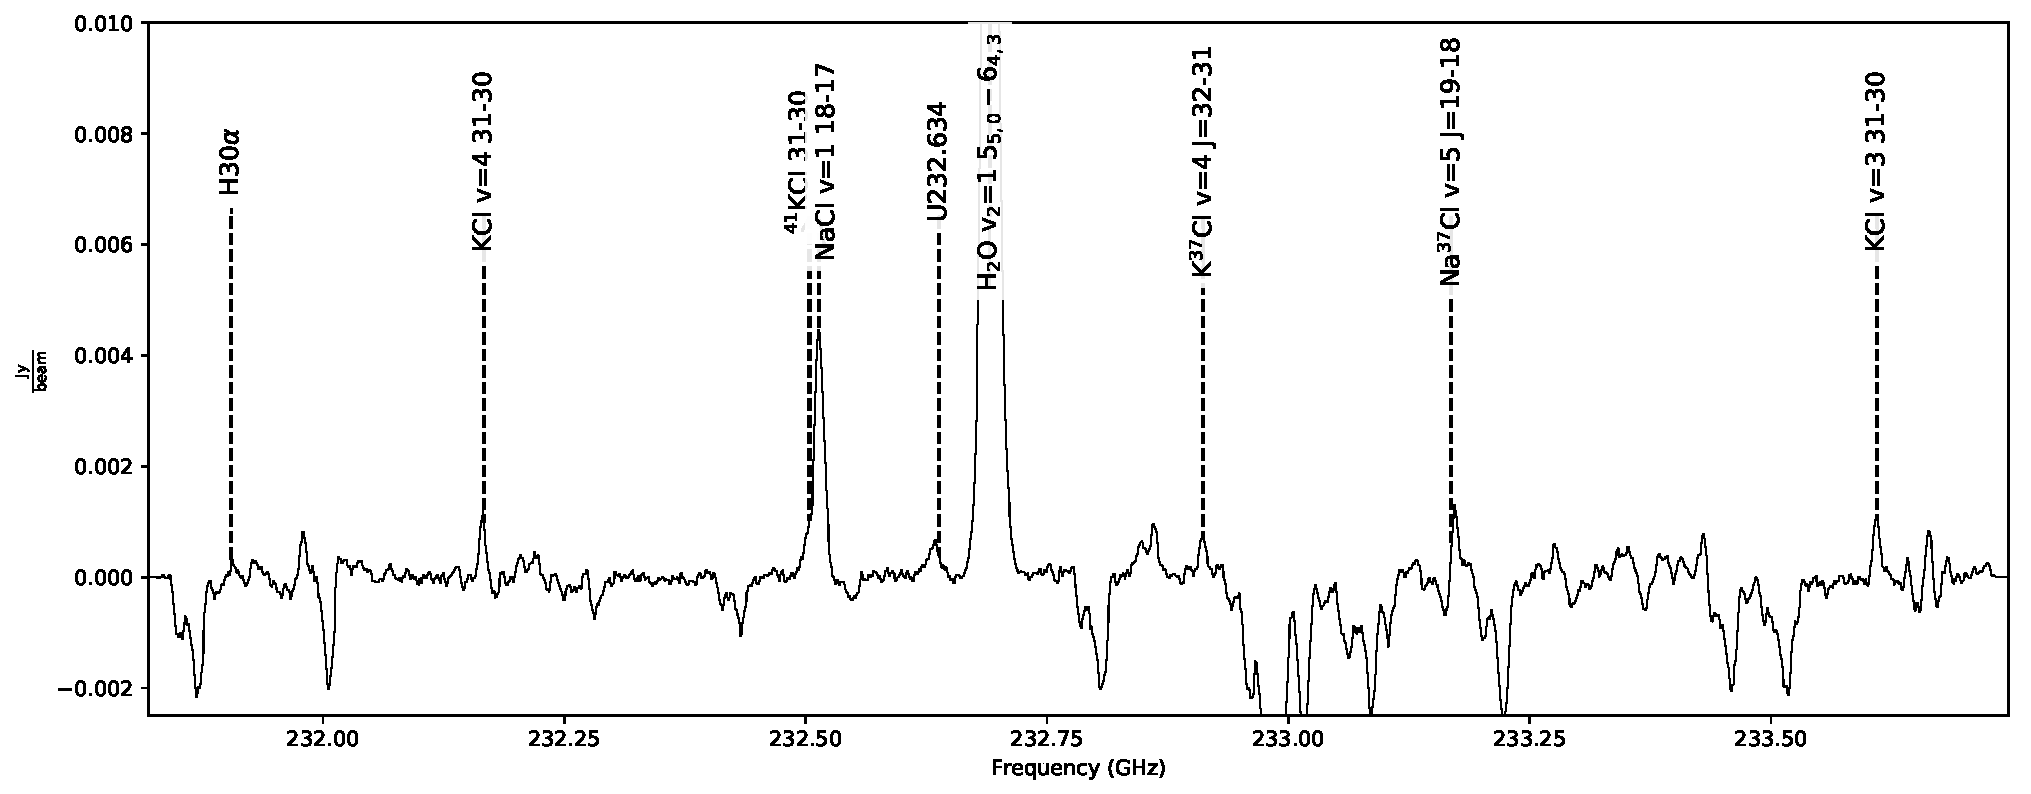
\includegraphics[scale=1,width=5.5in]{{figures/lines_labeled_OrionSourceI_B6_spw1_robust0.5}.pdf}
    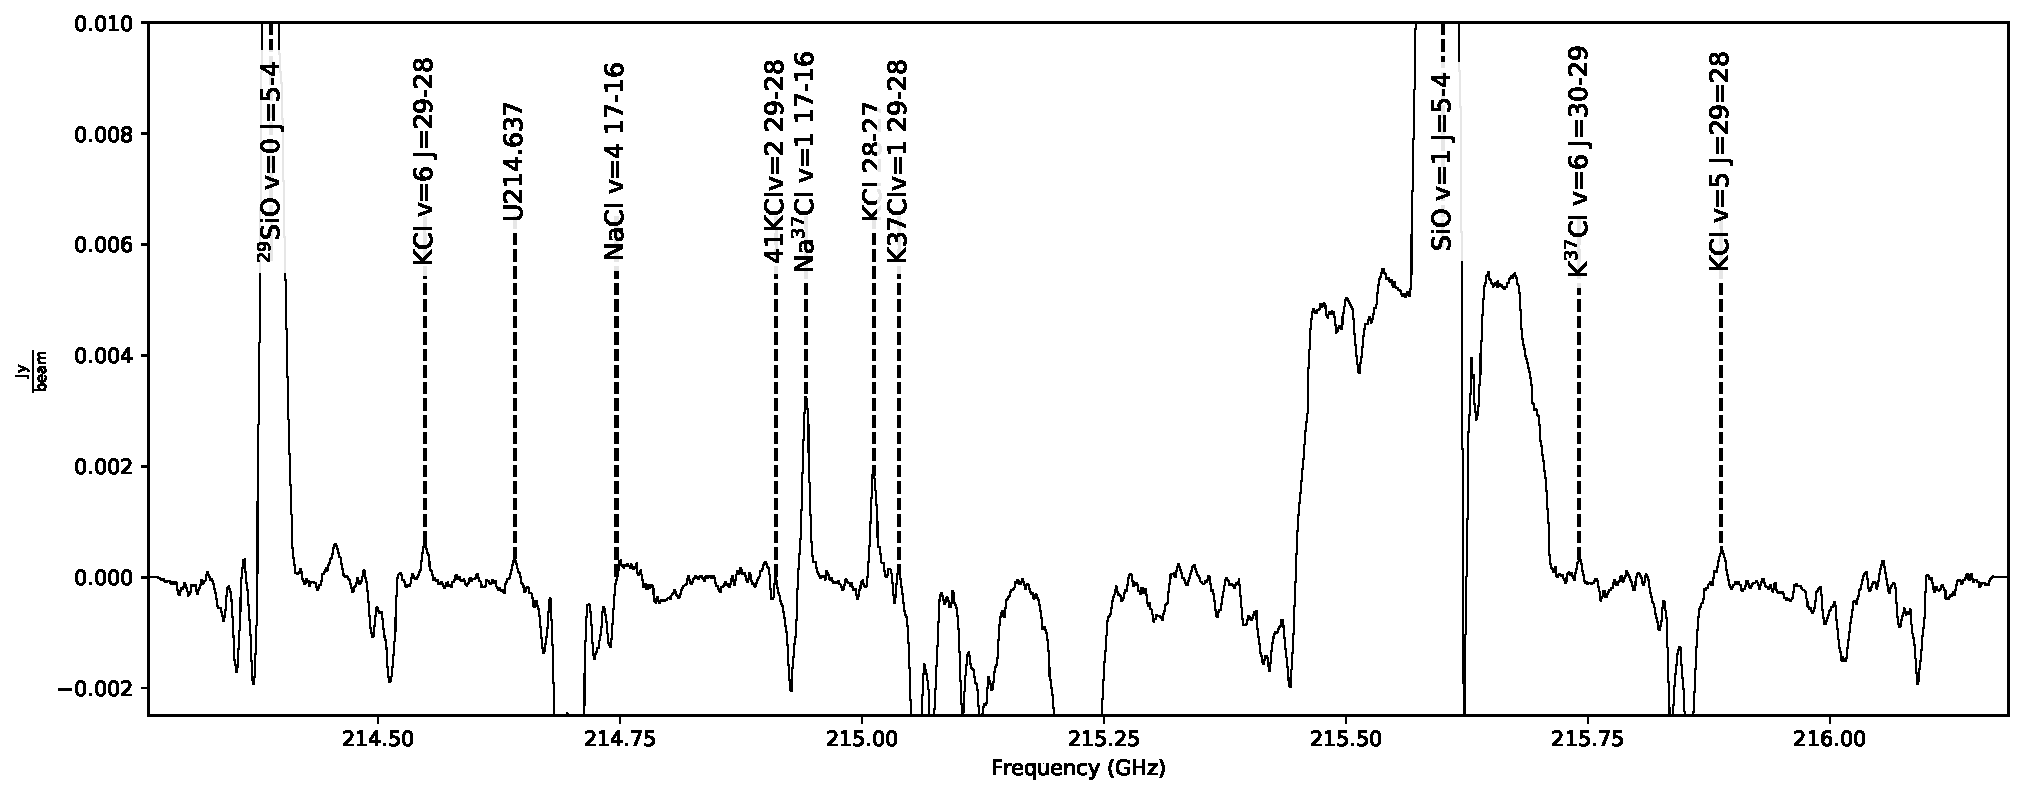
\includegraphics[scale=1,width=5.5in]{{figures/lines_labeled_OrionSourceI_B6_spw2_robust0.5}.pdf}
    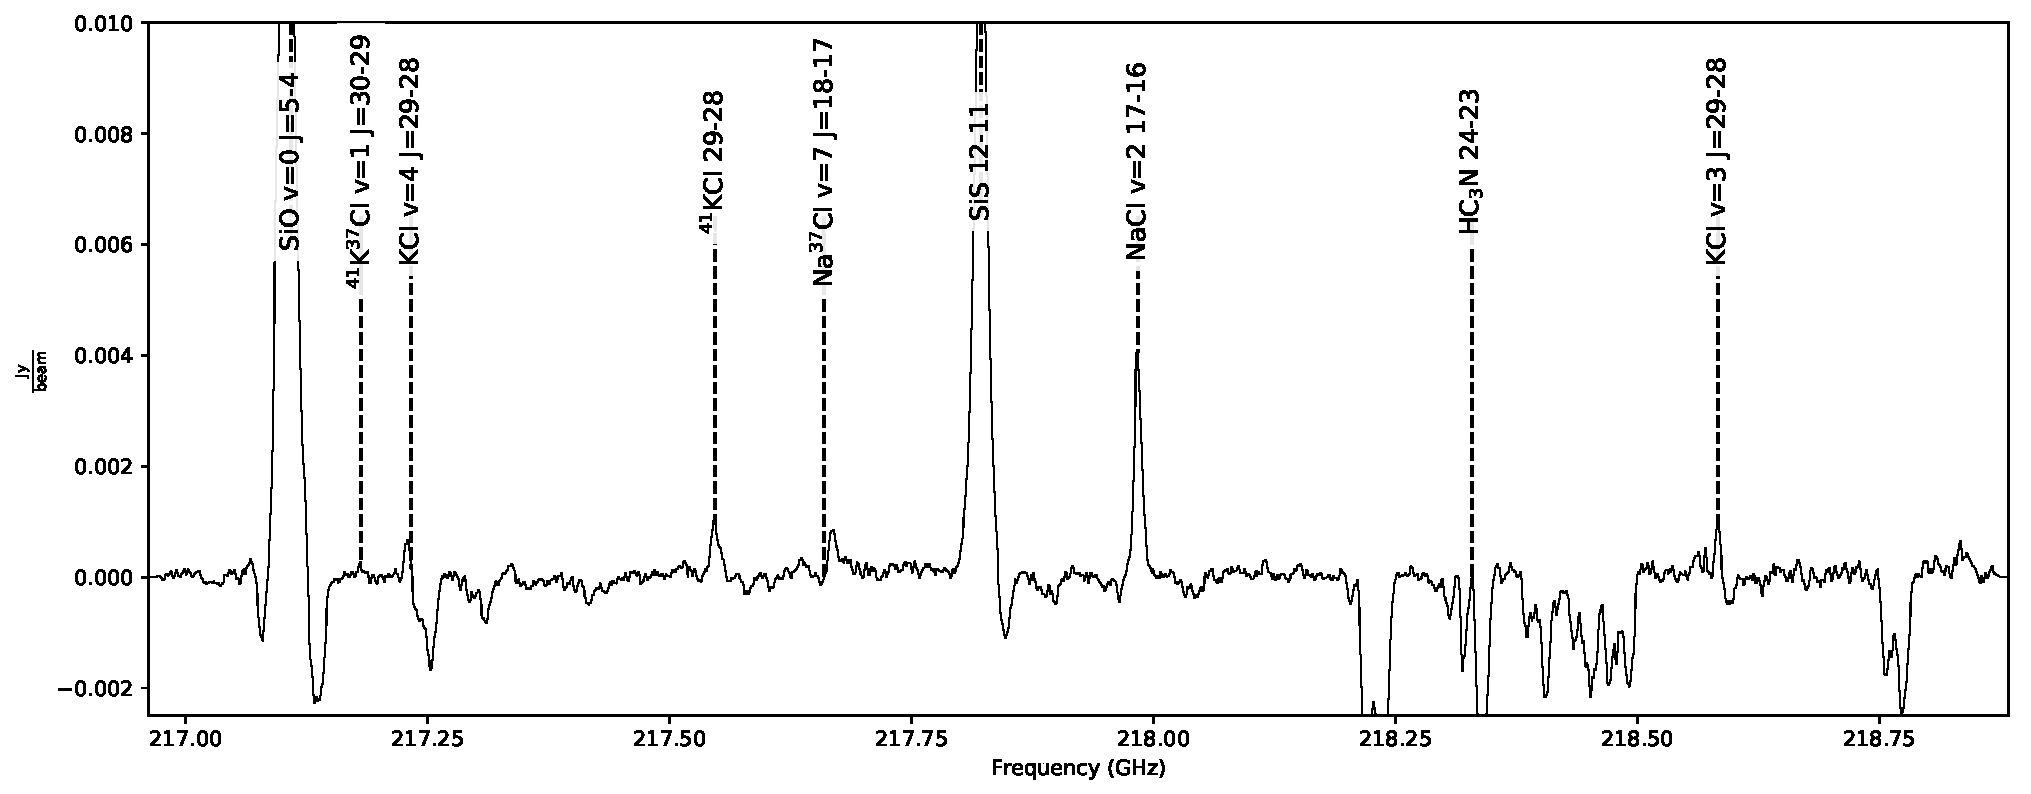
\includegraphics[scale=1,width=5.5in]{{figures/lines_labeled_OrionSourceI_B6_spw3_robust0.5}.pdf}
\caption{Stacked spectra B6}
\label{fig:spectrab6}
\end{figure*}
\begin{figure*}[!htp]
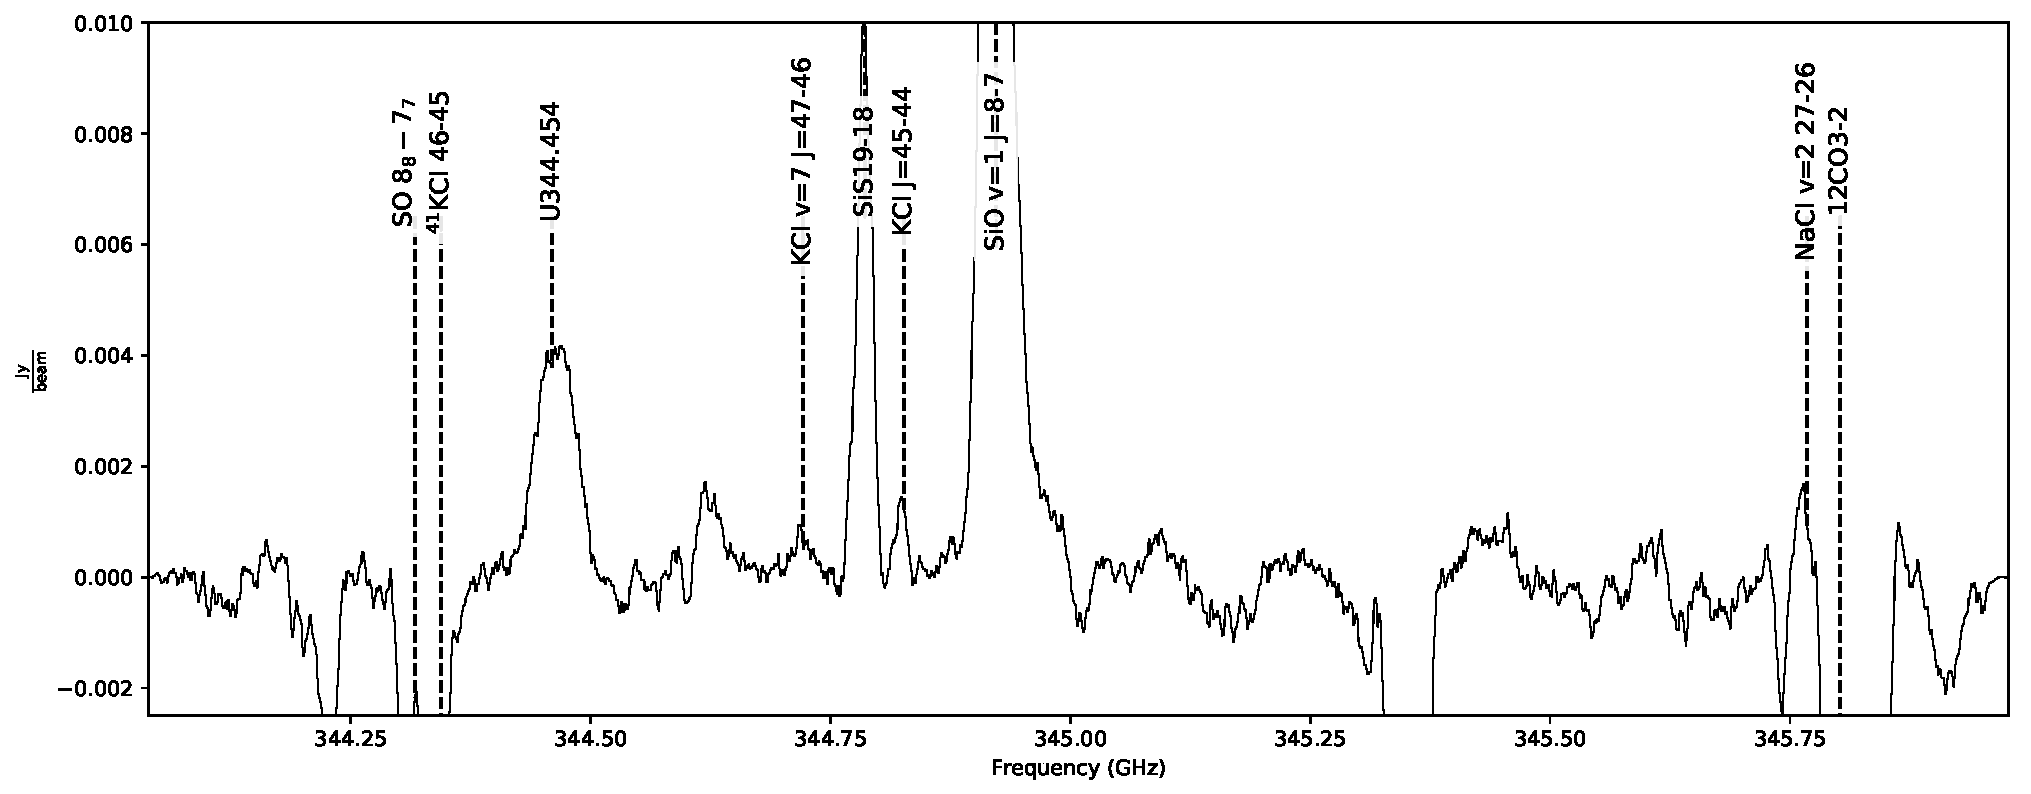
\includegraphics[scale=1,width=5.5in]{{figures/lines_labeled_OrionSourceI_B7.lb_spw0_robust0.5}.pdf}
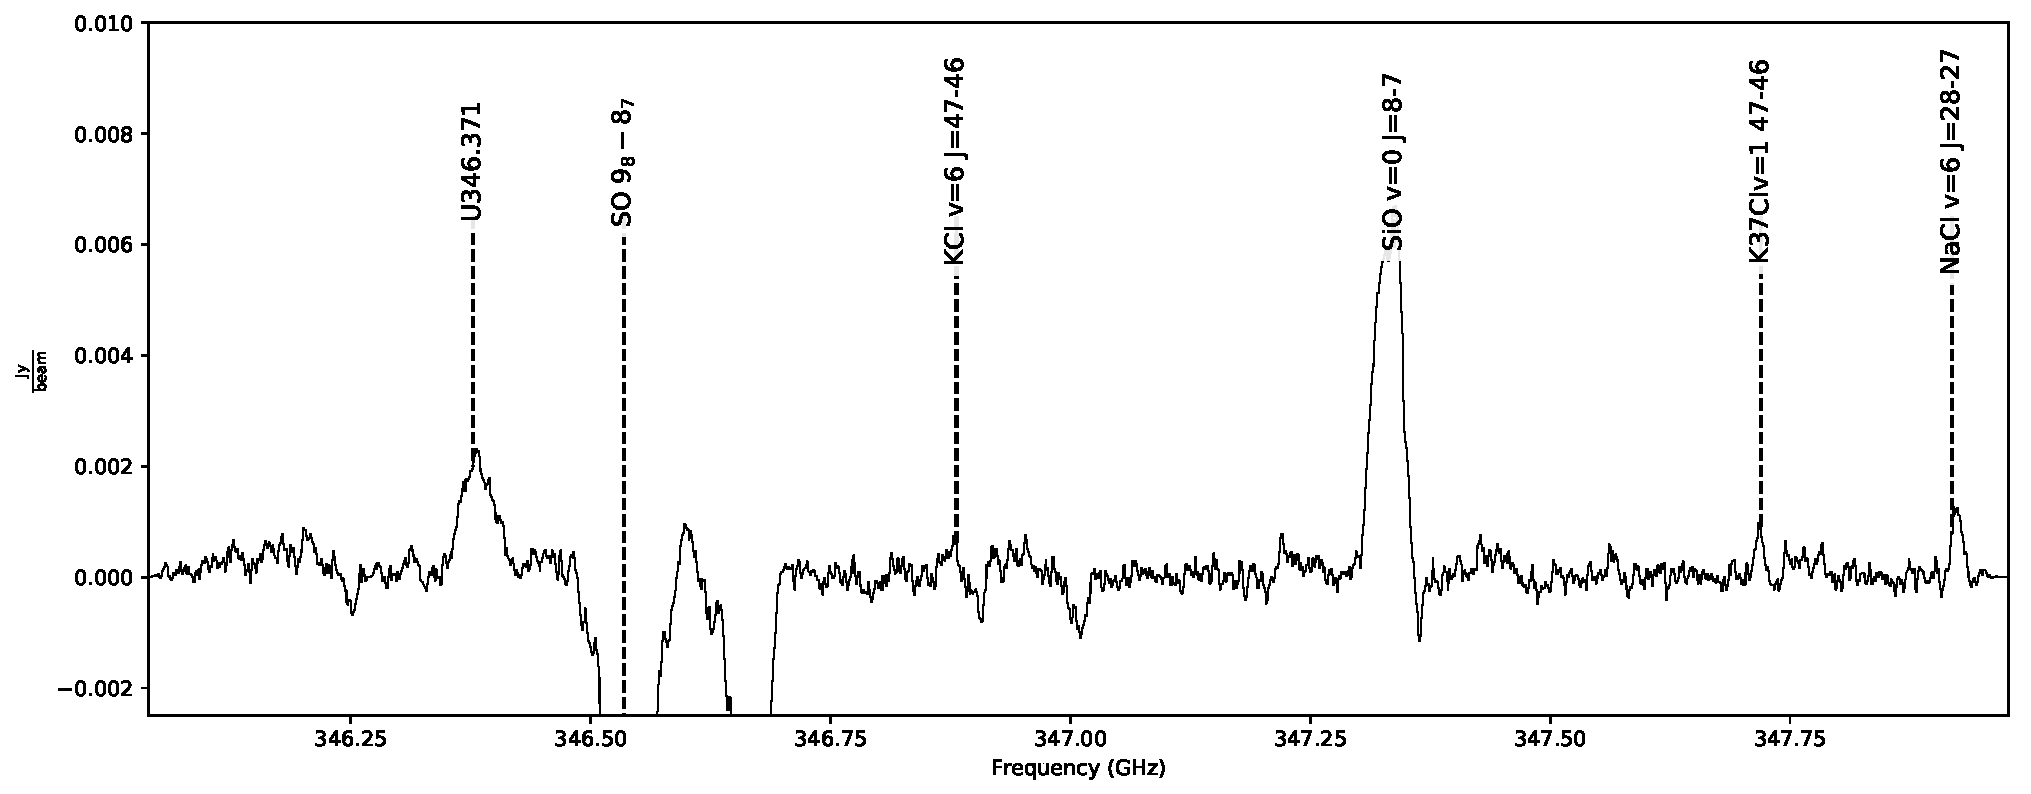
\includegraphics[scale=1,width=5.5in]{{figures/lines_labeled_OrionSourceI_B7.lb_spw1_robust0.5}.pdf}
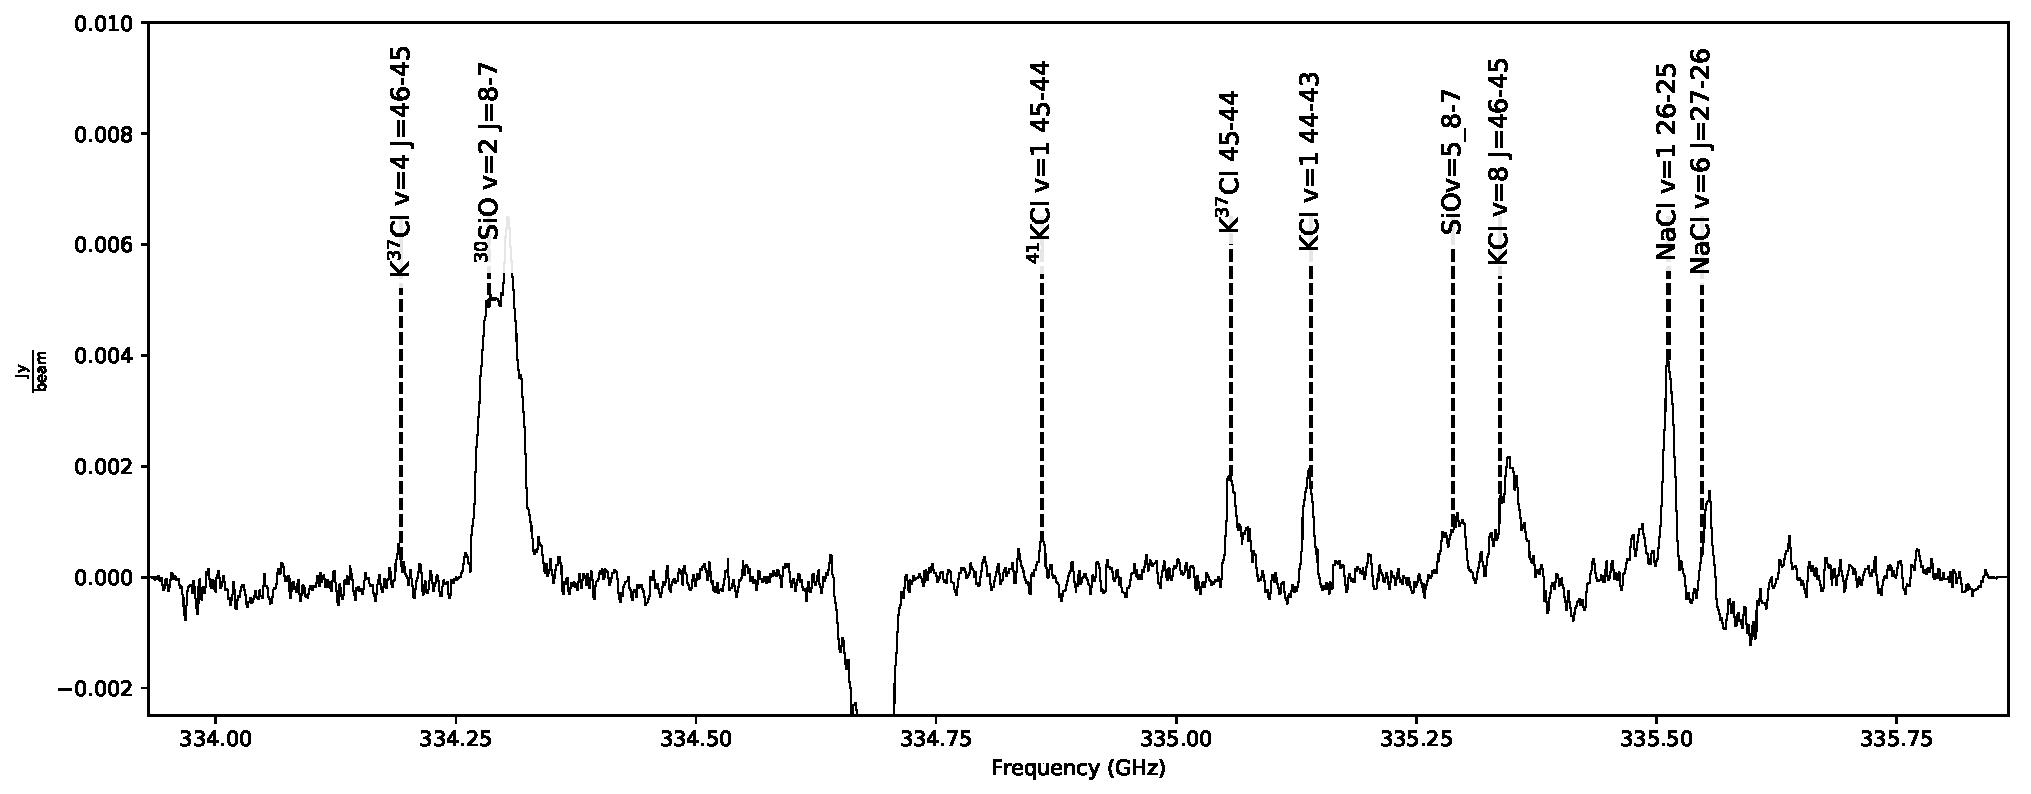
\includegraphics[scale=1,width=5.5in]{{figures/lines_labeled_OrionSourceI_B7.lb_spw2_robust0.5}.pdf}
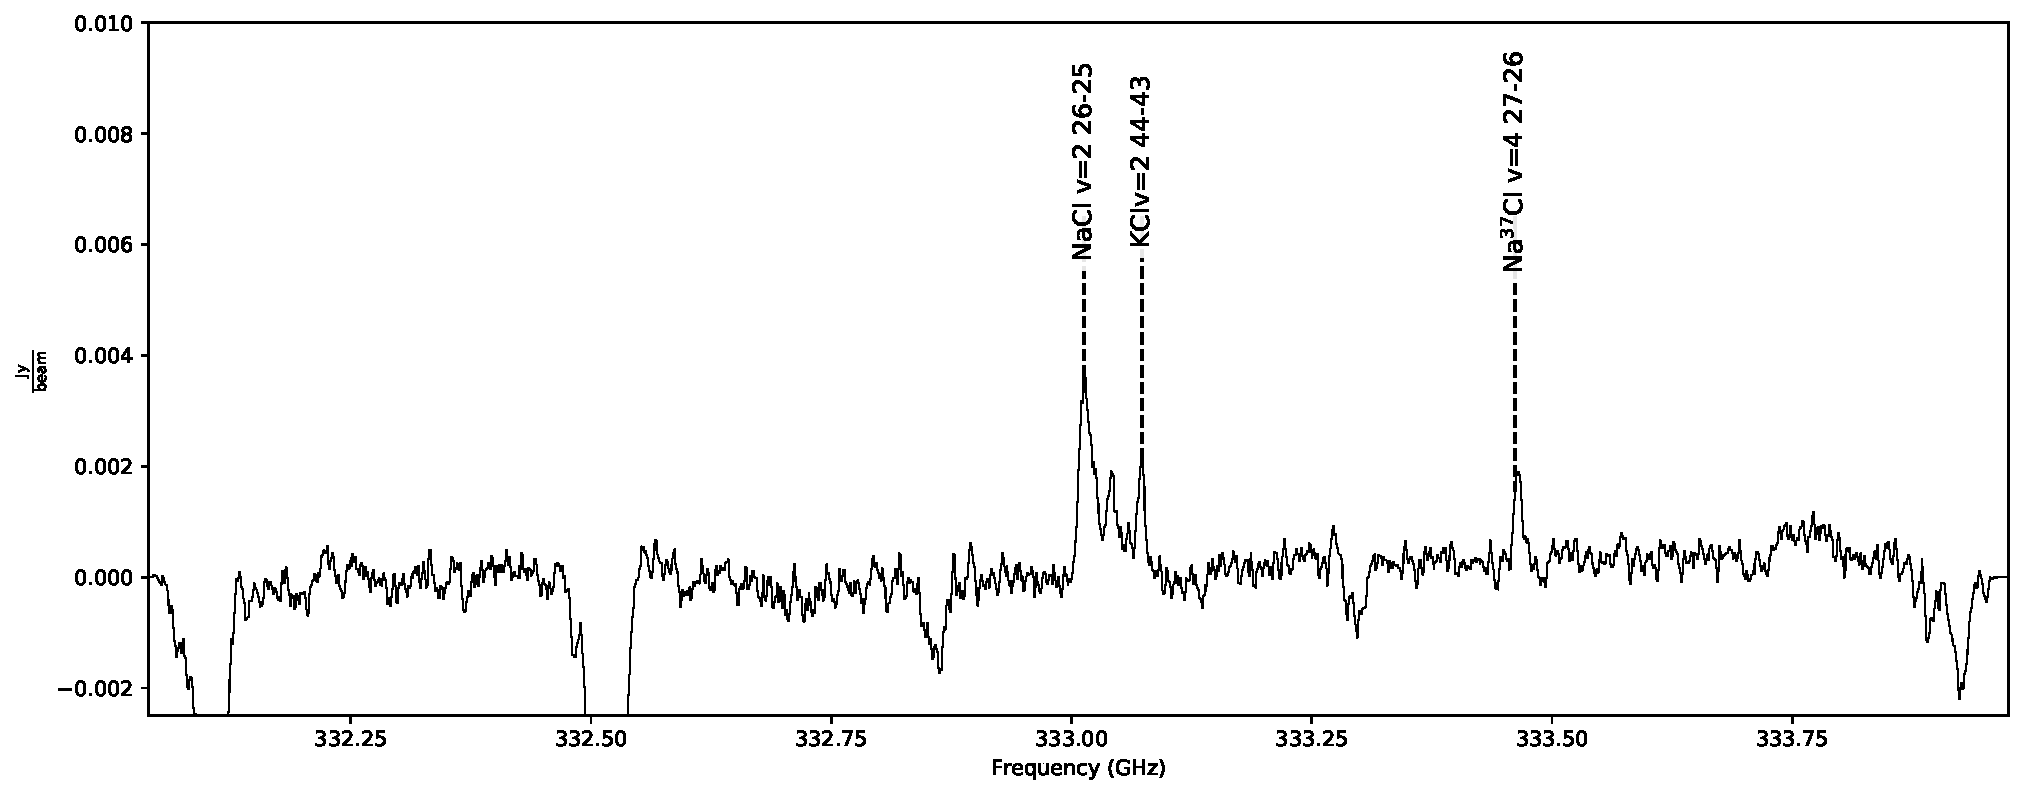
\includegraphics[scale=1,width=5.5in]{{figures/lines_labeled_OrionSourceI_B7.lb_spw3_robust0.5}.pdf}
\caption{Stacked spectra B7}
\label{fig:spectrab7}
\end{figure*}


In Tables \ref{tab:all_detections_B3}-\ref{tab:all_detections_B7}, we list all
of the salt lines in vibrational energy levels up to v=8 that lie within our
observed bands and whether or not they were detected.  We employ the following
flag scheme: `d' for detection, `n' for nondetection, `q' for questionable
(e.g., low signal-to-noise, but possibly detected, or in regions where the
noise is not Gaussian and may be affected by other lines).  We additionally
include a flag `c' for `confused', which we add to the flag string if the line
is blended with another brighter line of a different species.  There are robust
detections of about 60 lines, up to the v=6 vibrational level.

The majority of the NaCl and KCl lines that we detected are in excited
vibrational states.  Although transitions in higher vibrational states were
measured, and some reported, in \cite{Caris2004a}, these did not provide the
complete catalogs needed for this analysis, nor to our knowledge are these
catalogues available in any of the standard online databases: CDMS, SLAIM, JPL
\cite{Muller2005a,Lovas2005b,Pickett1998a}.  We obtained the KCl
frequencies for these lines from the catalogs of \cite{Barton2014a}, which was
designed primarily for use in exoplanet atmospheres and includes over 10$^5$
transitions for each molecular species and isotopologue with levels up to
$E_U\sim5\ee{4}$ K, and the NaCl frequencies from \cite{Cabezas2016a}, who
provided more accurate potential energy and dipole moment functions. The
primary result of these catalogs for the purposes of this work is the
prediction of frequencies in vibrational states higher than those measured in
the laboratory. 
% \rlp{Would it be fair just to say that we used Cabezas for the NaCl
% frequencies and Barton for the KCl frequencies?}

% The results of these works were then subsequently used by
% \citet{Barton2014a} to generate high-temperature line lists, primarily for use
% in exoplanet atmospheres, and includes over 10$^5$ transitions for each
% molecular species and isotopologue with levels up to $E_U\sim5\ee{4}$ K. The
% primary result for the purposes of this work is the prediction of frequencies
% in vibrational states higher than those measured in the laboratory. 

% We therefore used the predictions from the \citet{Barton2014a} catalog
% to identify lines with vibrational states $v>2$ for KCl and $v>4$ for NaCl.  
% \rlp{There's a paper by Cabezas et al, ApJ 2016 that claims to derive highly
% accurate frequencies, A coefficients, etc for NaCl up to J=150 and v=8; how
% does that fit into this story??}
% \ag{Added a reference.  Mostly, they fit the CDMS/SLAIM catalogs.  I've also switched
% to using the Cabezas values in the tables for NaCl.}

In using these catalogs, we found a systematic discrepancy between the rest
frequencies reported by Barton \cite{Barton2014a}, and those given by
\cite{Caris2004a} and \cite{Caris2002a} and the catalogs generated from them:
the KCl lines appear to be systematically offset by $\sim$15-20 \kms in the
Barton catalog.  
The Barton data are also discrepant with the more recent
\cite{Cabezas2016a} work that cataloged only NaCl lines
{\bf [rlp: is the NaCl offset also 15-20 \kms?]}. The offset is a
function of the vibrational and rotational energy states, indicating that it
resulted from an incorrect rotational and/or distortion constant.  We %correct
corrected the KCl data
for this error by performing a bilinear fit in frequency as a function of $v_u$
and $J_u$ to the transitions available in both \cite{Barton2014a} and
\cite{Caris2004a}; the resulting
frequency differences were generally $<0.1$ \kms, which is more than sufficient
for a reliable match to our observational spectra.  We then applied these
% and $J_u$.  In the transitions available in both catalogs the resulting
% frequency differences are generally $<0.1$ \kms, which is more than sufficient
% for a reliable match to our observational spectra.  We then applied these
fitted models to the higher-$v$ states tabulated by Barton to get corrected
rest frequencies for KCl.  % while for NaCl we used the \cite{Cabezas2016a}
% values. \rlp{we already said we used the Cabezas values for NaCl}  
We note that the values printed in \cite{Barton2014a} differ from
those in the digital catalogs hosted on \texttt{exomol.com}, so we suspect the
error was merely a transcription error of some sort.
%A more detailed re-fitting and prediction of the frequencies is beyond the
%scope of this \emph{Letter}, but is certainly warranted for follow-up efforts.

% \textbf{\color{red} At the moment, all of the line frequencies are shifted
% to higher frequencies by 17 \kms (KCl) and 3 \kms (NaCl) because of a discrepancy
% between the \cite{Barton2014a} catalog line frequencies and those of CDMS,
% JPL, and SLAIM.  The latter three, catalogued in Splatalogue, agree, and they
% agree better with my measurements.}

\begin{table*}[htp]
\centering
\caption{All observed lines in Band 3}
\begin{tabular}{cccccccc}
\label{tab:all_detections_B3}
Species & v & J$_u$ & J$_l$ & E$_U$ & A$_{ul}$ & Frequency & Flag \\
\hline
$^{41}$K$^{35}$Cl & 8 & 12 & 11 & 3092.4 & 0.00041 & 85.80766 & -n \\
$^{23}$Na$^{35}$Cl & 8 & 7 & 6 & 4035.4 & 0.00031 & 85.87018 & -n \\
$^{39}$K$^{37}$Cl & 7 & 12 & 11 & 2713.3 & 0.00041 & 85.87379 & -n \\
$^{41}$K$^{37}$Cl & 3 & 12 & 11 & 1183.9 & 0.00039 & 85.93776 & -n \\
$^{23}$Na$^{37}$Cl & 5 & 7 & 6 & 2538.2 & 0.00030 & 85.98167 & -d \\
$^{41}$K$^{35}$Cl & 7 & 12 & 11 & 2720.7 & 0.00042 & 86.33986 & cn \\
$^{39}$K$^{37}$Cl & 6 & 12 & 11 & 2339.4 & 0.00041 & 86.40364 & -n \\
$^{41}$K$^{37}$Cl & 2 & 12 & 11 & 801.6 & 0.00039 & 86.45668 & -n \\
$^{23}$Na$^{35}$Cl & 7 & 7 & 6 & 3550.1 & 0.00031 & 86.51754 & -q \\
$^{23}$Na$^{37}$Cl & 4 & 7 & 6 & 2043.6 & 0.00030 & 86.62109 & -d \\
$^{39}$K$^{35}$Cl & 10 & 12 & 11 & 3869.7 & 0.00044 & 86.68041 & -n \\
$^{41}$K$^{35}$Cl & 6 & 12 & 11 & 2345.7 & 0.00042 & 86.87413 & -n \\
$^{39}$K$^{37}$Cl & 5 & 12 & 11 & 1962.2 & 0.00042 & 86.93553 & -n \\
$^{41}$K$^{37}$Cl & 1 & 12 & 11 & 416.1 & 0.00040 & 86.97743 & -q \\
$^{23}$Na$^{35}$Cl & 6 & 7 & 6 & 3060.0 & 0.00032 & 87.16921 & -d \\
$^{39}$K$^{35}$Cl & 9 & 12 & 11 & 3500.3 & 0.00044 & 87.22792 & -n \\
$^{23}$Na$^{37}$Cl & 3 & 7 & 6 & 1544.3 & 0.00030 & 87.26464 & -d \\
$^{41}$K$^{35}$Cl & 5 & 12 & 11 & 1967.6 & 0.00042 & 87.41041 & -n \\
$^{39}$K$^{37}$Cl & 4 & 12 & 11 & 1581.9 & 0.00042 & 87.46938 & -n \\
$^{41}$K$^{37}$Cl & 0 & 12 & 11 & 27.3 & 0.00040 & 87.50010 & -q \\
$^{39}$K$^{35}$Cl & 8 & 12 & 11 & 3127.7 & 0.00044 & 87.77742 & -n \\
$^{23}$Na$^{35}$Cl & 5 & 7 & 6 & 2565.2 & 0.00032 & 87.82519 & -d \\
$^{23}$Na$^{37}$Cl & 2 & 7 & 6 & 1040.1 & 0.00031 & 87.91232 & -d \\
$^{41}$K$^{35}$Cl & 4 & 12 & 11 & 1586.3 & 0.00043 & 87.94866 & -n \\
$^{39}$K$^{37}$Cl & 3 & 12 & 11 & 1198.3 & 0.00042 & 88.00523 & -d \\
$^{39}$K$^{35}$Cl & 7 & 12 & 11 & 2751.8 & 0.00045 & 88.32895 & -q \\
$^{23}$Na$^{35}$Cl & 4 & 7 & 6 & 2065.5 & 0.00032 & 88.48549 & -d \\
$^{41}$K$^{35}$Cl & 3 & 12 & 11 & 1201.7 & 0.00043 & 88.48896 & cq \\
$^{39}$K$^{37}$Cl & 2 & 12 & 11 & 811.5 & 0.00042 & 88.54307 & -d \\
$^{23}$Na$^{37}$Cl & 1 & 7 & 6 & 531.1 & 0.00031 & 88.56415 & -d \\
$^{39}$K$^{35}$Cl & 6 & 12 & 11 & 2372.8 & 0.00045 & 88.88253 & -n \\
$^{41}$K$^{35}$Cl & 2 & 12 & 11 & 813.8 & 0.00043 & 89.03129 & -d \\
$^{39}$K$^{37}$Cl & 1 & 12 & 11 & 421.4 & 0.00043 & 89.08292 & -d \\
$^{23}$Na$^{35}$Cl & 3 & 7 & 6 & 1561.0 & 0.00033 & 89.15011 & -d \\
$^{41}$K$^{37}$Cl & 10 & 13 & 12 & 3776.8 & 0.00048 & 89.21871 & -n \\
$^{23}$Na$^{37}$Cl & 0 & 7 & 6 & 17.1 & 0.00031 & 89.22011 & -d \\
$^{39}$K$^{35}$Cl & 4 & 13 & 12 & 1609.5 & 0.00058 & 97.49133 & -d \\
$^{23}$Na$^{37}$Cl & 6 & 8 & 7 & 3032.7 & 0.00045 & 97.53449 & -q \\
$^{41}$K$^{35}$Cl & 0 & 13 & 12 & 32.8 & 0.00056 & 97.62809 & -d \\
$^{41}$K$^{37}$Cl & 7 & 14 & 13 & 2690.7 & 0.00061 & 97.85364 & -n \\
$^{39}$K$^{35}$Cl & 3 & 13 & 12 & 1220.6 & 0.00059 & 98.09753 & -d \\
$^{23}$Na$^{35}$Cl & 8 & 8 & 7 & 4040.1 & 0.00047 & 98.13295 & -q \\
$^{23}$Na$^{37}$Cl & 5 & 8 & 7 & 2542.9 & 0.00045 & 98.26052 & -q \\
$^{39}$K$^{37}$Cl & 10 & 14 & 13 & 3825.5 & 0.00064 & 98.33904 & -n \\
$^{41}$K$^{37}$Cl & 6 & 14 & 13 & 2321.0 & 0.00061 & 98.44993 & -n \\
$^{39}$K$^{35}$Cl & 2 & 13 & 12 & 828.3 & 0.00059 & 98.70595 & -d \\
$^{41}$K$^{35}$Cl & 10 & 14 & 13 & 3835.7 & 0.00065 & 98.86759 & cn \\
$^{23}$Na$^{35}$Cl & 7 & 8 & 7 & 3554.8 & 0.00047 & 98.87277 & -q \\
$^{39}$K$^{37}$Cl & 9 & 14 & 13 & 3461.0 & 0.00065 & 98.94969 & -n \\
$^{23}$Na$^{37}$Cl & 4 & 8 & 7 & 2048.4 & 0.00045 & 98.99127 & -d \\
$^{41}$K$^{37}$Cl & 5 & 14 & 13 & 1948.2 & 0.00062 & 99.04845 & -n \\
$^{39}$K$^{35}$Cl & 1 & 13 & 12 & 432.6 & 0.00059 & 99.31663 & -d \\
$^{41}$K$^{35}$Cl & 9 & 14 & 13 & 3470.3 & 0.00066 & 99.48329 & -n \\
$^{39}$K$^{37}$Cl & 8 & 14 & 13 & 3093.3 & 0.00065 & 99.56276 & -n \\
$^{23}$Na$^{35}$Cl & 6 & 8 & 7 & 3064.8 & 0.00048 & 99.61753 & -d \\
$^{41}$K$^{37}$Cl & 4 & 14 & 13 & 1572.3 & 0.00062 & 99.64924 & -n \\
$^{23}$Na$^{37}$Cl & 3 & 8 & 7 & 1549.1 & 0.00046 & 99.72675 & -d \\
$^{39}$K$^{35}$Cl & 0 & 13 & 12 & 33.6 & 0.00060 & 99.92952 & -d \\
$^{41}$K$^{35}$Cl & 8 & 14 & 13 & 3101.7 & 0.00066 & 100.10138 & -n \\
$^{39}$K$^{37}$Cl & 7 & 14 & 13 & 2722.6 & 0.00065 & 100.17822 & -n \\
$^{41}$K$^{37}$Cl & 3 & 14 & 13 & 1193.2 & 0.00063 & 100.25229 & -n \\
$^{23}$Na$^{35}$Cl & 5 & 8 & 7 & 2570.0 & 0.00048 & 100.36722 & -d \\
$^{23}$Na$^{37}$Cl & 2 & 8 & 7 & 1045.0 & 0.00046 & 100.46695 & -d \\
$^{41}$K$^{35}$Cl & 7 & 14 & 13 & 2730.0 & 0.00067 & 100.72190 & -n \\
$^{39}$K$^{37}$Cl & 6 & 14 & 13 & 2348.7 & 0.00066 & 100.79603 & -q \\
$^{41}$K$^{37}$Cl & 2 & 14 & 13 & 810.9 & 0.00063 & 100.85758 & -n \\
$^{39}$K$^{35}$Cl & 10 & 14 & 13 & 3879.0 & 0.00070 & 101.12088 & -n \\
$^{23}$Na$^{35}$Cl & 4 & 8 & 7 & 2070.4 & 0.00048 & 101.12183 & -d \\
$^{23}$Na$^{37}$Cl & 1 & 8 & 7 & 536.0 & 0.00047 & 101.21188 & -d \\
\hline
\end{tabular}

\par 
\end{table*}

\begin{table*}[htp]
\centering
\caption{All detected lines in Band 6}
\begin{tabular}{ccccccc}
\label{tab:all_detections_B6}
Species & v & J$_u$ & J$_l$ & E$_U$ & Frequency & Flag \\
\hline
$^{39}$K$^{37}$Cl & 7 & 30 & 29 & 2846.1 & 214.41527 & -n \\
$^{23}$Na$^{37}$Cl & 9 & 18 & 17 & 4547.4 & 214.43575 & cn \\
$^{39}$K$^{35}$Cl & 6 & 29 & 28 & 2499.6 & 214.54412 & -d \\
$^{41}$K$^{37}$Cl & 3 & 30 & 29 & 1316.8 & 214.57918 & -n \\
$^{23}$Na$^{35}$Cl & 4 & 17 & 16 & 2139.6 & 214.74036 & cn \\
$^{41}$K$^{35}$Cl & 2 & 29 & 28 & 940.8 & 214.90740 & cq \\
$^{23}$Na$^{37}$Cl & 1 & 17 & 16 & 606.5 & 214.93872 & -d \\
$^{39}$K$^{35}$Cl & 0 & 28 & 27 & 149.7 & 215.00828 & -d \\
$^{39}$K$^{37}$Cl & 1 & 29 & 28 & 548.5 & 215.03464 & cq \\
$^{41}$K$^{37}$Cl & 8 & 31 & 30 & 3187.6 & 215.09368 & cn \\
$^{41}$K$^{35}$Cl & 7 & 30 & 29 & 2854.2 & 215.57755 & cn \\
$^{39}$K$^{37}$Cl & 6 & 30 & 29 & 2473.0 & 215.73679 & -d \\
$^{41}$K$^{37}$Cl & 2 & 30 & 29 & 935.3 & 215.87559 & -n \\
$^{39}$K$^{35}$Cl & 5 & 29 & 28 & 2118.0 & 215.88373 & -d \\
$^{23}$Na$^{37}$Cl & 8 & 18 & 17 & 4072.5 & 216.04057 & -n \\
$^{39}$K$^{37}$Cl & 5 & 30 & 29 & 2096.7 & 217.06391 & -q \\
$^{41}$K$^{37}$Cl & 1 & 30 & 29 & 550.6 & 217.17723 & -q \\
$^{39}$K$^{35}$Cl & 4 & 29 & 28 & 1733.2 & 217.22891 & cd \\
$^{23}$Na$^{35}$Cl & 10 & 18 & 17 & 5070.5 & 217.31725 & cn \\
$^{39}$K$^{37}$Cl & 10 & 31 & 30 & 3957.2 & 217.47744 & -n \\
$^{41}$K$^{35}$Cl & 0 & 29 & 28 & 156.7 & 217.54317 & -d \\
$^{23}$Na$^{37}$Cl & 7 & 18 & 17 & 3593.1 & 217.65560 & -q \\
$^{41}$K$^{37}$Cl & 6 & 31 & 30 & 2452.9 & 217.72366 & -n \\
$^{39}$K$^{35}$Cl & 9 & 30 & 29 & 3635.2 & 217.79704 & cn \\
$^{23}$Na$^{35}$Cl & 2 & 17 & 16 & 1127.5 & 217.97998 & -d \\
$^{41}$K$^{35}$Cl & 5 & 30 & 29 & 2102.8 & 218.24805 & -n \\
$^{39}$K$^{37}$Cl & 4 & 30 & 29 & 1717.2 & 218.39657 & cn \\
$^{41}$K$^{37}$Cl & 0 & 30 & 29 & 162.6 & 218.48414 & cn \\
$^{39}$K$^{35}$Cl & 3 & 29 & 28 & 1345.1 & 218.57971 & -d \\
$^{41}$K$^{35}$Cl & 10 & 31 & 30 & 3968.1 & 218.64471 & -n \\
$^{39}$K$^{37}$Cl & 9 & 31 & 30 & 3593.5 & 218.82568 & -q \\
$^{23}$Na$^{37}$Cl & 0 & 18 & 17 & 104.6 & 229.24601 & -d \\
$^{39}$K$^{35}$Cl & 6 & 31 & 30 & 2521.2 & 229.29217 & cd \\
$^{23}$Na$^{35}$Cl & 10 & 19 & 18 & 5081.5 & 229.36540 & cn \\
$^{41}$K$^{35}$Cl & 2 & 31 & 30 & 962.5 & 229.68227 & cd \\
$^{23}$Na$^{37}$Cl & 7 & 19 & 18 & 3604.1 & 229.72316 & cn \\
$^{39}$K$^{37}$Cl & 1 & 31 & 30 & 570.2 & 229.81880 & -d \\
$^{41}$K$^{35}$Cl & 7 & 32 & 31 & 2875.9 & 229.90046 & -q \\
$^{39}$K$^{37}$Cl & 6 & 32 & 31 & 2494.7 & 230.07072 & -d \\
$^{41}$K$^{37}$Cl & 2 & 32 & 31 & 957.1 & 230.22070 & -q \\
$^{41}$K$^{37}$Cl & 7 & 33 & 32 & 2843.6 & 230.31852 & cn \\
$^{39}$K$^{35}$Cl & 0 & 30 & 29 & 171.4 & 230.32064 & -d \\
$^{39}$K$^{35}$Cl & 5 & 31 & 30 & 2139.8 & 230.72399 & -d \\
$^{23}$Na$^{35}$Cl & 2 & 18 & 17 & 1138.6 & 230.77883 & -d \\
$^{39}$K$^{35}$Cl & 10 & 32 & 31 & 4025.6 & 230.81309 & -n \\
$^{39}$K$^{35}$Cl & 4 & 31 & 30 & 1755.1 & 232.16185 & -d \\
$^{39}$K$^{35}$Cl & 9 & 32 & 31 & 3657.1 & 232.26613 & cn \\
$^{41}$K$^{35}$Cl & 0 & 31 & 30 & 178.7 & 232.49980 & cn \\
$^{23}$Na$^{35}$Cl & 1 & 18 & 17 & 625.2 & 232.50998 & -d \\
$^{41}$K$^{35}$Cl & 10 & 33 & 32 & 3990.1 & 232.69933 & cn \\
$^{41}$K$^{35}$Cl & 5 & 32 & 31 & 2124.8 & 232.74872 & -q \\
$^{23}$Na$^{35}$Cl & 8 & 19 & 18 & 4127.2 & 232.84920 & -q \\
$^{39}$K$^{37}$Cl & 9 & 33 & 32 & 3615.5 & 232.89230 & -n \\
$^{39}$K$^{37}$Cl & 4 & 32 & 31 & 1739.2 & 232.90755 & -d \\
$^{41}$K$^{37}$Cl & 10 & 34 & 33 & 3942.7 & 232.97243 & cn \\
$^{41}$K$^{37}$Cl & 0 & 32 & 31 & 184.6 & 233.00319 & cn \\
$^{41}$K$^{37}$Cl & 5 & 33 & 32 & 2102.9 & 233.12954 & cn \\
$^{23}$Na$^{37}$Cl & 5 & 19 & 18 & 2631.4 & 233.16458 & cd \\
$^{39}$K$^{35}$Cl & 3 & 31 & 30 & 1367.1 & 233.60570 & -d \\
$^{39}$K$^{35}$Cl & 8 & 32 & 31 & 3285.5 & 233.72540 & -n \\
\hline
\end{tabular}

\par 
\end{table*}

\begin{table*}[htp]
\centering
% \caption{All observed lines in Band 7}
% "observed" often means "detected", hence is misleading - Dick
\caption{Salt lines in Band 7}
\begin{tabular}{cccccccc}
\label{tab:all_detections_B7}
Species & v & J$_u$ & J$_l$ & E$_U$ & A$_{ul}$ & Frequency & Flag \\
\hline
$^{39}$K$^{37}$Cl & 5 & 46 & 45 & 2310.3 & 0.02398 & 332.14436 & cn \\
$^{39}$K$^{35}$Cl & 6 & 45 & 44 & 2712.4 & 0.02429 & 332.22193 & cq \\
$^{41}$K$^{37}$Cl & 8 & 48 & 47 & 3413.8 & 0.02483 & 332.29761 & -n \\
$^{41}$K$^{37}$Cl & 1 & 46 & 45 & 764.4 & 0.02295 & 332.34847 & -n \\
$^{41}$K$^{35}$Cl & 2 & 45 & 44 & 1154.0 & 0.02331 & 332.81369 & -n \\
$^{41}$K$^{35}$Cl & 9 & 47 & 46 & 3818.5 & 0.02527 & 332.83163 & -n \\
$^{23}$Na$^{35}$Cl & 2 & 26 & 25 & 1250.2 & 0.01800 & 333.00729 & -d \\
$^{39}$K$^{37}$Cl & 1 & 45 & 44 & 761.8 & 0.02309 & 333.01833 & cn \\
$^{23}$Na$^{35}$Cl & 7 & 27 & 26 & 3757.5 & 0.01900 & 333.03612 & cq \\
$^{39}$K$^{35}$Cl & 2 & 44 & 43 & 1155.3 & 0.02336 & 333.06770 & -d \\
$^{39}$K$^{37}$Cl & 8 & 47 & 46 & 3441.9 & 0.02504 & 333.10414 & -n \\
$^{39}$K$^{35}$Cl & 9 & 46 & 45 & 3849.6 & 0.02539 & 333.23510 & -n \\
$^{41}$K$^{37}$Cl & 4 & 47 & 46 & 1921.1 & 0.02398 & 333.43025 & -n \\
$^{23}$Na$^{37}$Cl & 4 & 27 & 26 & 2251.3 & 0.01800 & 333.45906 & -d \\
$^{41}$K$^{35}$Cl & 5 & 46 & 45 & 2317.6 & 0.02438 & 333.95245 & -n \\
$^{39}$K$^{37}$Cl & 4 & 46 & 45 & 1932.1 & 0.02415 & 334.18696 & -n \\
$^{39}$K$^{35}$Cl & 5 & 45 & 44 & 2332.2 & 0.02446 & 334.29930 & -d \\
$^{41}$K$^{37}$Cl & 7 & 48 & 47 & 3049.3 & 0.02501 & 334.32791 & cd \\
$^{41}$K$^{37}$Cl & 0 & 46 & 45 & 377.7 & 0.02311 & 334.35249 & cn \\
$^{41}$K$^{35}$Cl & 1 & 45 & 44 & 764.9 & 0.02347 & 334.85439 & -d \\
$^{41}$K$^{35}$Cl & 8 & 47 & 46 & 3452.1 & 0.02545 & 334.89960 & -n \\
$^{41}$K$^{37}$Cl & 10 & 49 & 48 & 4149.6 & 0.02605 & 335.04657 & cn \\
$^{39}$K$^{37}$Cl & 0 & 45 & 44 & 370.4 & 0.02325 & 335.05072 & -d \\
$^{39}$K$^{35}$Cl & 1 & 44 & 43 & 761.7 & 0.02353 & 335.13396 & -d \\
$^{39}$K$^{37}$Cl & 7 & 47 & 46 & 3073.3 & 0.02522 & 335.16416 & -q \\
$^{39}$K$^{35}$Cl & 8 & 46 & 45 & 3479.1 & 0.02557 & 335.33093 & cq \\
$^{41}$K$^{37}$Cl & 3 & 47 & 46 & 1544.2 & 0.02414 & 335.45237 & -n \\
$^{23}$Na$^{35}$Cl & 1 & 26 & 25 & 737.2 & 0.01800 & 335.50656 & -d \\
$^{23}$Na$^{35}$Cl & 6 & 27 & 26 & 3269.0 & 0.01900 & 335.54793 & cq \\
$^{23}$Na$^{37}$Cl & 8 & 28 & 27 & 4211.3 & 0.02000 & 335.63074 & cn \\
$^{41}$K$^{35}$Cl & 7 & 48 & 47 & 3099.1 & 0.02730 & 344.08981 & cn \\
$^{41}$K$^{35}$Cl & 0 & 46 & 45 & 389.0 & 0.02525 & 344.33834 & cn \\
$^{39}$K$^{37}$Cl & 6 & 48 & 47 & 2718.1 & 0.02705 & 344.35234 & cn \\
$^{41}$K$^{37}$Cl & 2 & 48 & 47 & 1180.5 & 0.02589 & 344.60998 & cq \\
$^{39}$K$^{35}$Cl & 7 & 47 & 46 & 3122.1 & 0.02747 & 344.71476 & -d \\
$^{41}$K$^{35}$Cl & 10 & 49 & 48 & 4214.6 & 0.02843 & 344.73191 & -n \\
$^{39}$K$^{35}$Cl & 0 & 45 & 44 & 381.2 & 0.02534 & 344.82061 & -d \\
$^{39}$K$^{37}$Cl & 9 & 49 & 48 & 3840.1 & 0.02817 & 345.02524 & -n \\
$^{23}$Na$^{35}$Cl & 7 & 28 & 27 & 3774.1 & 0.02100 & 345.31422 & cn \\
$^{41}$K$^{35}$Cl & 3 & 47 & 46 & 1572.6 & 0.02637 & 345.37541 & cn \\
$^{41}$K$^{37}$Cl & 5 & 49 & 48 & 2327.8 & 0.02698 & 345.40918 & cn \\
$^{39}$K$^{35}$Cl & 10 & 48 & 47 & 4249.6 & 0.02864 & 345.42961 & cn \\
$^{39}$K$^{37}$Cl & 2 & 47 & 46 & 1182.6 & 0.02612 & 345.59885 & cn \\
$^{23}$Na$^{37}$Cl & 4 & 28 & 27 & 2267.9 & 0.02000 & 345.75480 & cn \\
$^{23}$Na$^{35}$Cl & 2 & 27 & 26 & 1266.8 & 0.02000 & 345.76204 & cd \\
$^{39}$K$^{35}$Cl & 3 & 46 & 45 & 1578.4 & 0.02650 & 345.94809 & cn \\
$^{41}$K$^{35}$Cl & 6 & 48 & 47 & 2726.5 & 0.02750 & 346.22022 & -n \\
$^{39}$K$^{37}$Cl & 5 & 48 & 47 & 2343.3 & 0.02724 & 346.47449 & -n \\
$^{41}$K$^{37}$Cl & 1 & 48 & 47 & 797.3 & 0.02607 & 346.69248 & cn \\
$^{39}$K$^{35}$Cl & 6 & 47 & 46 & 2745.3 & 0.02767 & 346.87489 & -d \\
$^{41}$K$^{35}$Cl & 9 & 49 & 48 & 3851.5 & 0.02863 & 346.87825 & cn \\
$^{39}$K$^{37}$Cl & 8 & 49 & 48 & 3474.8 & 0.02837 & 347.16340 & -n \\
$^{41}$K$^{35}$Cl & 2 & 47 & 46 & 1187.0 & 0.02655 & 347.49773 & -q \\
$^{41}$K$^{37}$Cl & 4 & 49 & 48 & 1954.1 & 0.02717 & 347.50839 & -n \\
$^{23}$Na$^{37}$Cl & 8 & 29 & 28 & 4228.0 & 0.02200 & 347.55955 & -n \\
$^{39}$K$^{35}$Cl & 9 & 48 & 47 & 3882.6 & 0.02884 & 347.60673 & -n \\
$^{39}$K$^{37}$Cl & 1 & 47 & 46 & 794.8 & 0.02630 & 347.71265 & -d \\
$^{23}$Na$^{35}$Cl & 6 & 28 & 27 & 3285.7 & 0.02100 & 347.91891 & nc \\
\hline
\end{tabular}

\par 
\end{table*}


%The low observed brightness temperatures suggest that the emission from
%these lines is optically thin.

We have fit Gaussian line profiles to each of the transitions we flagged as
`detected' in Tables \ref{tab:all_detections_B3}-\ref{tab:all_detections_B7}.
The fits are reported in Tables
\ref{tab:NaCl_salt_lines}-\ref{tab:41K37Cl_salt_lines}.  Some of these
measurements (e.g., of the KCl v=5 45-44 line) are discrepantly
high, suggesting that they are blends with other species as denoted in 
Tables \ref{tab:all_detections_B3}-\ref{tab:all_detections_B7}.


\section{Spatial distribution of the salt emission}
\label{sec:wherefrom}
In \sourcei, the salt lines originate from the surface layers of the disk (the Band 7
lines exhibit NaCl emission peaks at $\pm0.032\arcsec=13$ AU above the disk),
% \citet{Ginsburg2018b} showed that these species come only from the disk's
% immediate surroundings, 
unlike SiO and \water that both exhibit high vertical extents consistent with
outflow \cite{Ginsburg2018b}.  No emission in the salt lines is observed
toward the optically thick continuum in the disk midplane (Figure
\ref{fig:spatial}).  Although the carriers of the lines were unassigned at the
time, \cite{Ginsburg2018b} modeled the line emission now assigned to these
salts as a
truncated Keplerian disk, finding that the radial distribution of the emission
has an inner cutoff $\approx35-40$ AU and an outer cutoff $\approx55-60$~AU.

% ((constants.sigma_sb * 4 * np.pi * (35*u.au)**2 / (1e4*u.L_sun))**(-1/4)).decompose()
% <Quantity 665.33595877 K>
% ((constants.sigma_sb * 4 * np.pi * (60*u.au)**2 / (1e4*u.L_sun))**(-1/4)).decompose()
% <Quantity 508.15873227 K>
The equilibrium temperature in this radius range can be computed assuming the central
source has a luminosity $L=10^4 \lsun = 4 \pi r^2 \sigma_{SB} T^4 $, where we
solve for temperature with $r$ at the inner and outer radius, giving $T_{eq} =
508-665$ K for $r=35-60$ AU, assuming the disk intercepts all of the starlight 
at this radius.  More realistically, providing the opposite limiting case,
$T_{eq}=120-185$ K for a flat disk \cite{Chiang1997a}.  These cooler temperatures
are consistent with the observed brightness temperatures in the outer
part of the continuum disk (in Figure \ref{fig:spatial}, the NaCl emission
begins just beyond the $T=300$ K contour), although the temperature in the inner
portion of the disk reaches $>500$ K.

\begin{figure*}[!htp]
    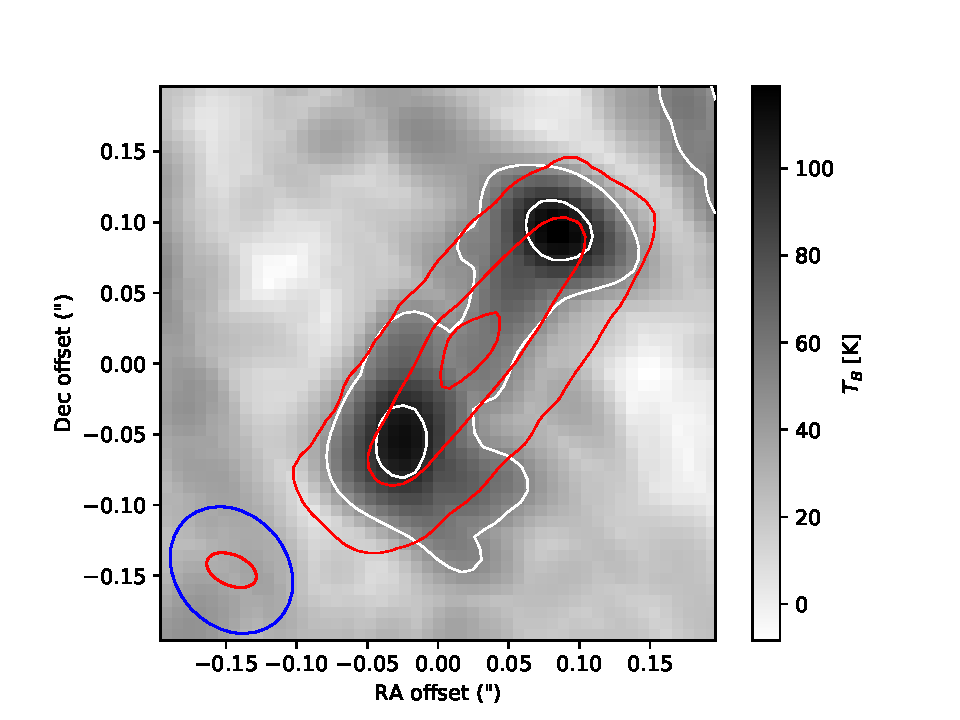
\includegraphics[scale=1,width=2.0in]{{figures/OrionSourceI_NaClv=3_7-6_robust0.5.maskedclarkclean10000_medsub_K_peak_offset_contours}.pdf}
    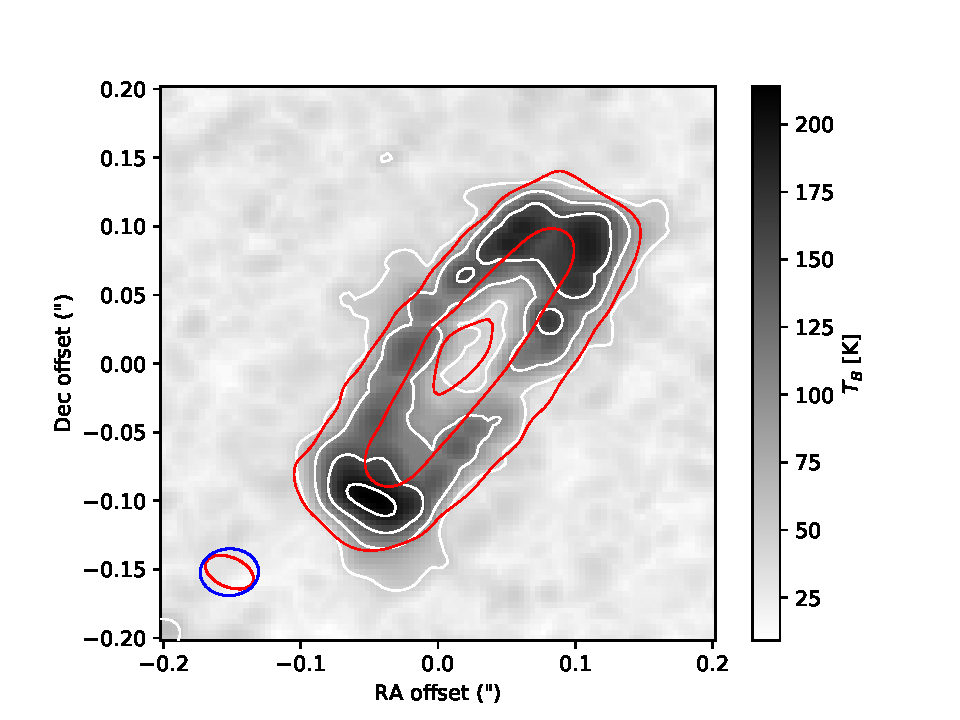
\includegraphics[scale=1,width=2.0in]{{figures/OrionSourceI_NaClv=1_18-17_robust0.5.maskedclarkclean10000_medsub_K_peak_offset_contours}.pdf}
    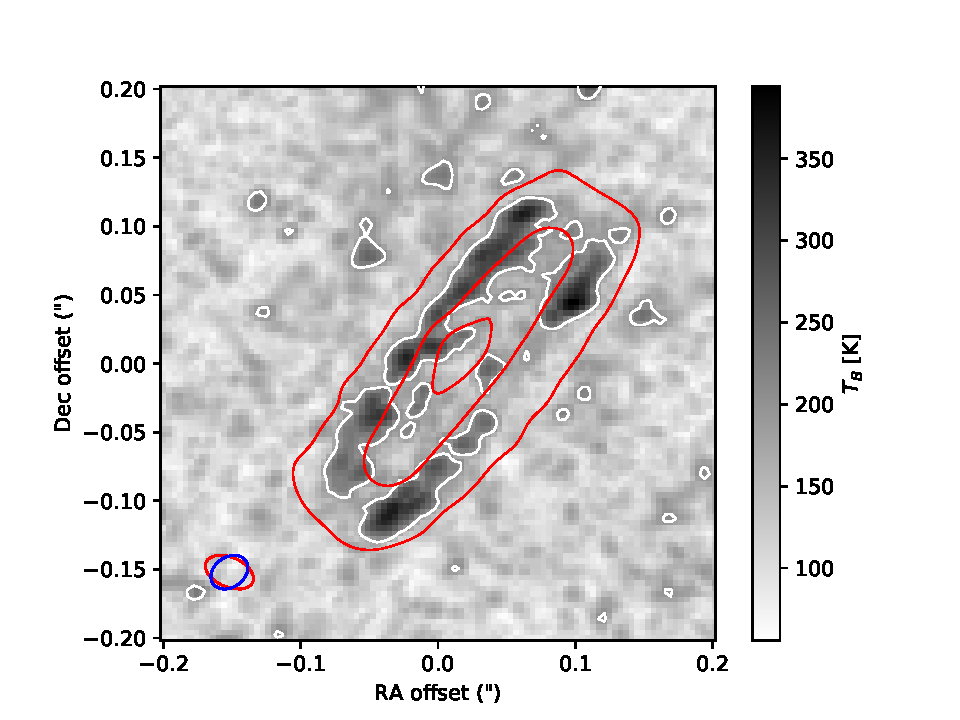
\includegraphics[scale=1,width=2.0in]{{figures/OrionSourceI_NaClv=2_26-25_robust0.5.maskedclarkclean10000_medsub_K_peak_offset_contours}.pdf}
\caption{Peak intensity images of NaCl lines in each band showing the spatial
distribution of the emission.  From left to right, the lines are: 87.26 GHz
NaCl v=3 J=7-6, 232.51 GHz NaCl v=1 J=18-17, and 333.01 GHz NaCl v=2 J=26-25.
These are the brightest uncontaminated lines in each of their observing bands.
The red contours show the Band 6 226 GHz continuum at levels of 50, 300, and 500 K.
White contours are shown at 50, 100, and 150 K.
The red and blue ellipses show the beams for the continuum and the line emission,
respectively.  The beam sizes are
$0.10 \arcsec \times 0.08 \arcsec$, PA $40.6 \degrees$,
$0.043 \arcsec \times 0.034 \arcsec$, PA $-87.4 \degrees$, and
$0.029 \arcsec \times 0.022 \arcsec$, PA $-54.6 \degrees$, respectively.
}
\label{fig:spatial}
\end{figure*}

We also compare the salt emission locations to the SiO emission regions.
Figure \ref{fig:sioonnacl} shows the \mbox{SiO v=0 J=8-7} line, which is
thermally excited (it shows no sign of masing at any velocity) and traces the
outflow.  The \mbox{SiO v=5 J=8-7} line, with an upper state energy level of
8747 K, is also shown.  It clearly traces a smaller radius than the NaCl line,
but a similar height in the disk.  By contrast, the \mbox{SiO v=0 J=8-7}
emission, with $E_U=75$ K, starts above the vertical centroid of the NaCl line.
These spatial anticorrelations suggest that the difference between the
molecules' emission patterns is driven partly by excitation, since the salt
lines have upper state energy levels intermediate between the SiO v=0 and v=5
states and trace an intermediate region.

% \bam{This reads
% as a result, not as discussion, as there's no conclusion drawn here.  What does
% this result tell us?  Seems like we're saying that the production method for
% SiO and NaCl/KCl probably aren't the same - they aren't co-located, so it's
% probably not shock/outflow-induced for NaCl/KCl?  This runs contrary to what is
% said later on in the discussion, however.}
% \ag{Added a conclusion.}


%\begin{figure*}[!htp]
%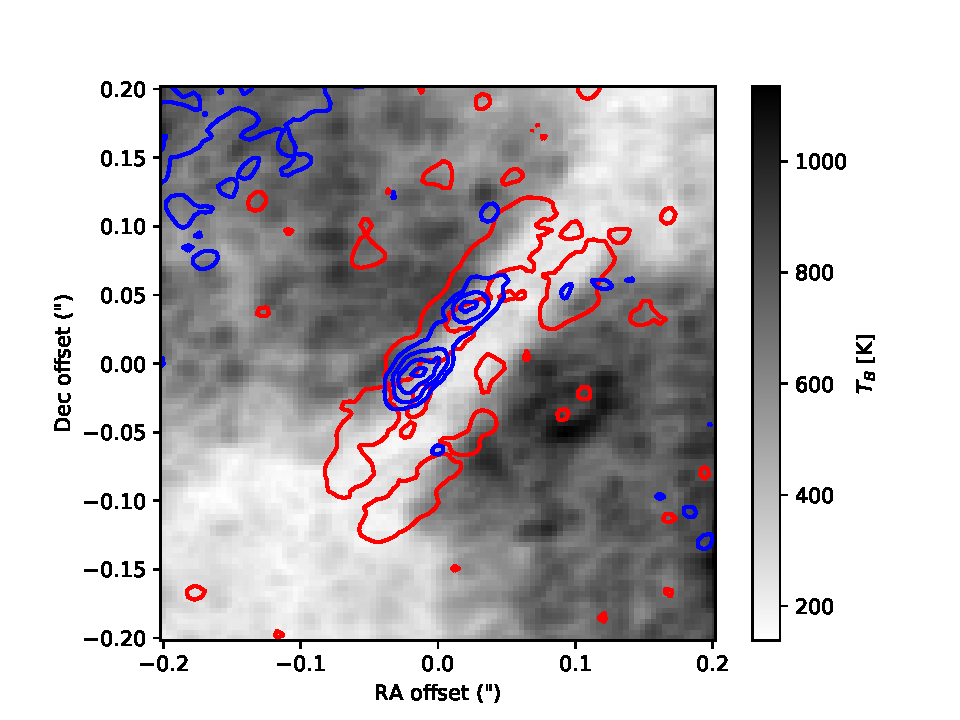
\includegraphics[scale=1,width=4in]{figures/SiO_8-7_on_NaClv=2_26-25.pdf}
%\caption{Peak intensity map of SiO v=0 J=8-7 (gray scale), NaCl v=2 J=26-25
%(red contour; 200 K) and {SiO v=5 J=8-7} (blue contours; 300, 400, 500, and 600
%K).  The blue contours in the upper-left come from a blend with a different
%line.
%}
%\label{fig:sioonnacl}
%\end{figure*}


% This estimate provides the expected temperature of
% gas at the surface of a passive disk in this radius range. {\color{red}We could
% obtain more realistic temperature estimates using the \citet{Chiang1997a}
% approximations for a flat or flared disk.}

\begin{table*}[htp]
\centering
\caption{NaCl Lines}
\begin{tabular}{ccccccc}
\label{tab:NaCl_salt_lines}
 J$_u$ & J$_l$ & Frequency & Velocity & Amplitude & $\int T_A dv$ & E$_U$ \\
  &  & $\mathrm{GHz}$ & $\mathrm{km\,s^{-1}}$ & $\mathrm{K}$ & $\mathrm{K\,km\,s^{-1}}$ & $\mathrm{K}$ \\
\hline
&\vspace{-0.75em}\\
\multicolumn{7}{c}{$v = 1$} \\
\vspace{-0.75em}\\ 
 26 & 25 & 335.50656 & 5.5 (0.1) & 29.1 (0.8) & 339.9 (5.4) & 737.2 \\
 18 & 17 & 232.50998 & 5.4 (0.2) & 23.9 (0.7) & 396.6 (6.7) & 625.7 \\
&\vspace{-0.75em}\\
\multicolumn{7}{c}{$v = 2$} \\
\vspace{-0.75em}\\
 17 & 16 & 217.98023 & 5.2 (0.1) & 19.3 (0.4) & 267.8 (3.6) & 1128.4 \\
 18 & 17 & 230.77917 & 5.6 (0.1) & 19.3 (0.4) & 297.7 (3.7) & 1139.5 \\
 26 & 25 & 333.00729 & 7.4 (0.3) & 21.7 (0.9) & 352.2 (8.9) & 1250.2 \\
 27 & 26 & 345.76204 & 0.2 (0.9) & 11.5 (1.9) & 136.4 (13.8) & 1266.8 \\
&\vspace{-0.75em}\\
\multicolumn{7}{c}{$v = 3$} \\
\vspace{-0.75em}\\
 7 & 6 & 89.15011 & 3.8 (0.5) & 14.1 (1.1) & 183.1 (9.0) & 1561.0 \\
&\vspace{-0.75em}\\
\multicolumn{7}{c}{$v = 4$} \\
\vspace{-0.75em}\\
 7 & 6 & 88.48549 & 3.8 (0.7) & 11.4 (1.0) & 185.4 (10.5) & 2065.5 \\
 8 & 7 & 101.12183 & 3.1 (0.3) & 15.5 (0.8) & 214.1 (7.0) & 2070.4 \\
&\vspace{-0.75em}\\
\multicolumn{7}{c}{$v = 5$} \\
\vspace{-0.75em}\\
 8 & 7 & 100.36722 & 3.7 (0.5) & 10.0 (0.9) & 122.3 (6.6) & 2570.0 \\
 7 & 6 & 87.82519 & 4.5 (0.6) & 11.6 (1.1) & 173.8 (9.9) & 2565.2 \\
&\vspace{-0.75em}\\
\multicolumn{7}{c}{$v = 6$} \\
\vspace{-0.75em}\\
 8 & 7 & 99.61753 & 4.4 (0.7) & 7.7 (0.9) & 100.0 (6.8) & 3064.8 \\
 7 & 6 & 87.16921 & 3.4 (1.2) & 7.2 (1.8) & 73.9 (11.4) & 3060.0 \\
\hline
\end{tabular}

\par 
\end{table*}

\begin{table*}[htp]
\centering
\caption{Na$^{37}$Cl Lines}
\begin{tabular}{ccccccc}
\label{tab:Na37Cl_salt_lines}
 J$_u$ & J$_l$ & Frequency & Velocity & Width & Amplitude & E$_U$ \\
  &  & $\mathrm{GHz}$ & $\mathrm{km\,s^{-1}}$ & $\mathrm{km\,s^{-1}}$ & $\mathrm{K}$ & $\mathrm{K}$ \\
\hline
&\vspace{-0.75em}\\
\multicolumn{7}{c}{$v = 0$} \\
\vspace{-0.75em}\\
 7 & 6 & 89.22066 & 2.5 (0.4) & 5.0 (0.4) & 18.2 (1.2) & 17.1 \\
&\vspace{-0.75em}\\
\multicolumn{7}{c}{$v = 1$} \\
\vspace{-0.75em}\\
 31 & 30 & 229.81801 & 6.5 (0.3) & 4.8 (0.3) & 7.2 (0.4) & 570.2 \\
 26 & 25 & 335.50625 & 5.8 (0.1) & 4.7 (0.1) & 29.1 (0.8) & 736.8 \\
&\vspace{-0.75em}\\
\multicolumn{7}{c}{$v = 2$} \\
\vspace{-0.75em}\\
 26 & 25 & 333.00524 & 9.0 (0.3) & 6.2 (0.3) & 21.9 (0.9) & 1249.3 \\
&\vspace{-0.75em}\\
\multicolumn{7}{c}{$v = 3$} \\
\vspace{-0.75em}\\
 12 & 11 & 88.00457 & 6.6 (1.4) & 6.3 (1.4) & 5.7 (1.1) & 1198.3 \\
&\vspace{-0.75em}\\
\multicolumn{7}{c}{$v = 4$} \\
\vspace{-0.75em}\\
 27 & 26 & 333.45280 & 11.0 (0.5) & 4.4 (0.5) & 11.3 (1.0) & 2249.5 \\
 8 & 7 & 98.98970 & 9.3 (1.1) & 4.1 (1.1) & 8.3 (1.9) & 2046.6 \\
&\vspace{-0.75em}\\
\multicolumn{7}{c}{$v = 5$} \\
\vspace{-0.75em}\\
 7 & 6 & 87.82328 & 10.5 (0.6) & 5.2 (0.7) & 12.1 (1.2) & 2563.0 \\
 29 & 28 & 215.88296 & 7.3 (2.1) & 4.3 (2.1) & 3.0 (1.3) & 2118.0 \\
\hline
\end{tabular}

\par 
\end{table*}

\begin{table*}[htp]
\centering
\caption{KCl Lines}
\begin{tabular}{ccccccc}
\label{tab:KCl_salt_lines}
 J$_u$ & J$_l$ & Frequency & Velocity & Width & Amplitude & E$_U$ \\
  &  & $\mathrm{GHz}$ & $\mathrm{km\,s^{-1}}$ & $\mathrm{km\,s^{-1}}$ & $\mathrm{K}$ & $\mathrm{K}$ \\
\hline
&\vspace{-0.75em}\\
\multicolumn{7}{c}{$v = 0$} \\
\vspace{-0.75em}\\
 28 & 27 & 215.00828 & 5.5 (0.6) & 4.3 (0.6) & 10.4 (1.3) & 149.7 \\
 30 & 29 & 230.32064 & 4.6 (0.2) & 4.8 (0.2) & 14.4 (0.4) & 171.4 \\
 45 & 44 & 344.82061 & 2.5 (1.1) & 4.9 (1.1) & 9.7 (1.8) & 381.2 \\
 13 & 12 & 99.92952 & 4.0 (0.3) & 4.8 (0.3) & 15.3 (0.9) & 33.6 \\
&\vspace{-0.75em}\\
\multicolumn{7}{c}{$v = 1$} \\
\vspace{-0.75em}\\
 44 & 43 & 335.13396 & 3.3 (0.3) & 4.1 (0.3) & 14.1 (0.8) & 761.7 \\
&\vspace{-0.75em}\\
\multicolumn{7}{c}{$v = 2$} \\
\vspace{-0.75em}\\
 13 & 12 & 98.70595 & 2.0 (0.8) & 6.4 (0.8) & 14.2 (1.5) & 828.3 \\
&\vspace{-0.75em}\\
\multicolumn{7}{c}{$v = 3$} \\
\vspace{-0.75em}\\
 13 & 12 & 98.09753 & 6.1 (1.1) & 5.0 (1.1) & 9.2 (1.7) & 1220.6 \\
 29 & 28 & 218.57971 & 4.4 (0.4) & 3.3 (0.4) & 5.0 (0.6) & 1345.1 \\
&\vspace{-0.75em}\\
\multicolumn{7}{c}{$v = 4$} \\
\vspace{-0.75em}\\
 13 & 12 & 97.49133 & 8.0 (2.1) & 7.0 (2.4) & 6.1 (1.5) & 1609.5 \\
 29 & 28 & 217.22891 & -0.3 (0.6) & 3.2 (0.6) & 3.5 (0.6) & 1733.2 \\
&\vspace{-0.75em}\\
\multicolumn{7}{c}{$v = 5$} \\
\vspace{-0.75em}\\
 31 & 30 & 230.72399 & 5.3 (0.4) & 4.3 (0.4) & 5.2 (0.5) & 2139.8 \\
 29 & 28 & 215.88373 & 6.3 (2.1) & 4.3 (2.1) & 3.0 (1.3) & 2118.0 \\
&\vspace{-0.75em}\\
\multicolumn{7}{c}{$v = 6$} \\
\vspace{-0.75em}\\
 47 & 46 & 346.87489 & 0.7 (1.1) & 5.5 (1.2) & 4.4 (0.8) & 2745.3 \\
 29 & 28 & 214.54412 & 6.3 (1.9) & 4.4 (1.9) & 3.4 (1.3) & 2499.6 \\
\hline
\end{tabular}

\par 
\end{table*}

\begin{table*}[htp]
\centering
\caption{K$^{37}$Cl Lines}
\begin{tabular}{ccccccccc}
\label{tab:K37Cl_salt_lines}
QNs & Frequency & Velocity & Velocity error & Width & Width error & Amplitude & Amplitude error & E$_U$ \\
 & $\mathrm{GHz}$ & $\mathrm{km\,s^{-1}}$ & $\mathrm{km\,s^{-1}}$ & $\mathrm{km\,s^{-1}}$ & $\mathrm{km\,s^{-1}}$ & $\mathrm{K}$ & $\mathrm{K}$ & $\mathrm{K}$ \\
\hline
v=3-3 J=12-11 & 88.00457 & 6.6 & 1.4 & 6.3 & 1.4 & 5.7 & 1.1 & 1198.3 \\
v=2-2 J=12-11 & 88.54225 & 8.0 & 1.5 & 4.6 & 1.5 & 4.3 & 1.2 & 811.5 \\
v=1-1 J=12-11 & 89.08229 & 5.2 & 1.2 & 4.7 & 1.2 & 5.5 & 1.2 & 421.4 \\
v=6-6 J=30-29 & 215.73578 & 7.3 & 2.8 & 3.0 & 2.8 & 1.9 & 1.5 & 2473.0 \\
v=1-1 J=31-30 & 229.81801 & 6.5 & 0.3 & 4.8 & 0.3 & 7.2 & 0.4 & 570.2 \\
v=6-6 J=32-31 & 230.06943 & 5.6 & 1.3 & 5.1 & 1.3 & 1.9 & 0.4 & 2494.7 \\
v=4-4 J=32-31 & 232.90536 & 7.8 & 1.1 & 5.1 & 1.1 & 4.0 & 0.7 & 1739.2 \\
v=0-0 J=45-44 & 335.05221 & 6.2 & 0.4 & 6.4 & 0.4 & 12.1 & 0.7 & 370.4 \\
v=1-1 J=47-46 & 347.71265 & 4.6 & 0.5 & 3.4 & 0.5 & 7.4 & 1.0 & 794.8 \\
\hline
\end{tabular}

\par 
\end{table*}

\begin{table*}[htp]
\centering
\caption{$^{41}$KCl Lines}
\begin{tabular}{ccccccc}
\label{tab:41KCl_salt_lines}
 J$_u$ & J$_l$ & Frequency & Velocity & Width & Amplitude & E$_U$ \\
  &  & $\mathrm{GHz}$ & $\mathrm{km\,s^{-1}}$ & $\mathrm{km\,s^{-1}}$ & $\mathrm{K}$ & $\mathrm{K}$ \\
\hline
&\vspace{-0.75em}\\
\multicolumn{7}{c}{$v = 0$} \\
\vspace{-0.75em}\\
0 & 29 & 28 & 217.54351 & 5.0 (0.7) & 6.5 (0.7) & 4.5 (0.4) & 156.7 \\
 13 & 12 & 97.62803 & 4.9 (2.5) & 10.0 (3.2) & 6.5 (1.3) & 32.8 \\
&\vspace{-0.75em}\\
\multicolumn{7}{c}{$v = 2$} \\
\vspace{-0.75em}\\
 7 & 6 & 87.91199 & 5.3 (0.6) & 6.0 (0.6) & 13.3 (1.1) & 1039.3 \\
\hline
\end{tabular}

\par 
\end{table*}

\begin{table*}[htp]
\centering
\caption{$^{41}$K$^{37}$Cl Lines}
\begin{tabular}{ccccccc}
\label{tab:41K37Cl_salt_lines}
 J$_u$ & J$_l$ & Frequency & Velocity & Width & Amplitude & E$_U$ \\
  &  & $\mathrm{GHz}$ & $\mathrm{km\,s^{-1}}$ & $\mathrm{km\,s^{-1}}$ & $\mathrm{K}$ & $\mathrm{K}$ \\
\hline
\hline
&\vspace{-0.75em}\\
\multicolumn{7}{c}{$v = 7$} \\
\vspace{-0.75em}\\
 48 & 47 & 334.32791 & -9.5 (0.0) & 5.7 (0.3) & 24.5 (0.9) & 3049.3 \\
\end{tabular}

\par 
\end{table*}








\section{Excitation}
The detection of vibrationally excited transitions from v=0 to v=6 at similar
brightness suggests that the vibrational excitation temperature $T_{ex,vib}$ of
the molecules is high.  However, we see sharply decreasing populations in
the higher rotational levels, indicating a much lower $T_{ex,rot}$.
% Since the
% molecules are not characterized by a single $T_{ex}$, they may be excited by
% some non-thermal mechanism.

% We detect highly excited transitions of NaCl and KCl, many with Einstein A
% coefficients in the range $\sim0.01-0.1$ s$^{-1}$, suggesting they are
% radiatively rather than collisionally excited.

% These high excitation lines
% are unlikely to be excited by collisions, since the gas would have to be hot
% enough to excite molecules into states with $E_U > 2000$ K and would therefore
% likely be hot enough to dissociate the molecules {\color{red} It would be nice
% to back this up with numbers}.  Alternately, at high densities and more
% moderate temperatures, the salts would likely be absorbed into dust grains.

% We calculate the level population as
% \begin{equation}
%     N_u = \frac{8 \pi \nu k_B}{g_u c^2 h A_{ul}} \int T_A d\nu
% %    nline = 8 * np.pi * freq * constants.k_B / constants.h / Aul / constants.c**2
% %    # term2 = np.exp(-constants.h*freq/(constants.k_B*Tex)) -1
% %    # term2 -> kt / hnu
% %    # kelvin-hertz
% %    Khz = (kkms * (freq/constants.c)).to(u.K * u.MHz)
% %    return (nline * Khz / degeneracies).to(u.cm**-2)
% \end{equation}
% {\color{red} (this is mostly a sanity check)}

Within each vibrational state for which we observed several transitions, we attempt
to measure a rotational temperature.  For the KCl v=0 state, in which we have
detected 4 rotational transitions from $30 < E_U < 400$ K, the best fit
is $T_{rot}\sim105$ K (Figure
\ref{fig:rotationdiagrams}).  At such a low temperature, the populations of the
vibrationally excited states should be effectively zero.  

Similarly, for each rotational transition observed from multiple vibrational
levels, we measure a vibrational temperature.  We find values that range from
1000-5000 K, although these fits are subject to very large
uncertainties.
% the fits are consistent with any temperature within this range.
% (and, statistically but not physically, they are consistent with arbitrarily
% large excitation temperatures).  
There are also statistically significant
outliers from the single-temperature model, suggesting that the level
populations may not be well-characterized by a single temperature.

\begin{figure*}[!htp]
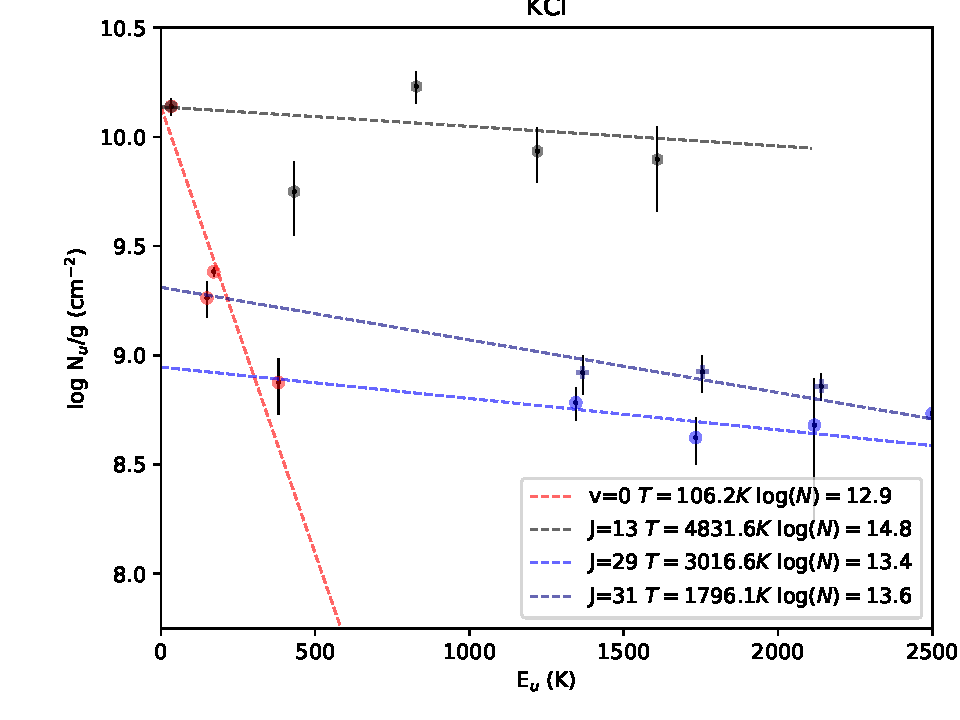
\includegraphics[scale=1,width=3.5in]{figures/KCl_rotational_diagrams.pdf}
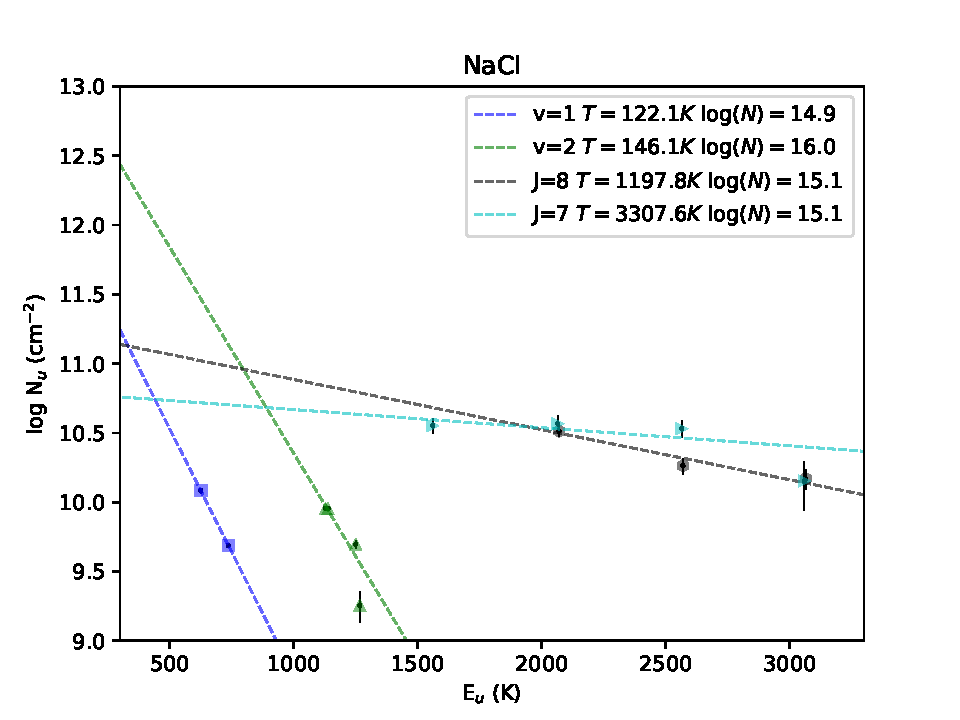
\includegraphics[scale=1,width=3.5in]{figures/NaCl_rotational_diagrams.pdf}
\caption{Rotational energy diagrams for the KCl and NaCl lines.  While each
vibrational state can internally be explained reasonably well by a single
consistent rotation temperature in the range $T_{rot}\sim50-150$ K, the population
distribution between vibrational excitation states cannot.}
\label{fig:rotationdiagrams}
\end{figure*}

% The rotational temperatures are reasonably consistent with the lower bound
% disk temperatures at this radius, hinting that the salt emission lines are
% coming from somewhere below the surface of the disk.  If this is the case,
% there are likely to be few optical photons reaching the salt molecules,
% since those are readily absorbed by the small grains in the upper layers.


% Since the highest clearly detected energy state detected has $E_U\sim3000$ K
% (see Table \ref{tab:all_detections_B3}; the v=6 lines of NaCl have three
% J-transitions detected), the radiation field likely turns over at around this
% temperature, implying the presence of a slightly cooler radiation field than
% implied in \citet{Testi2010a}, but still much warmer than the equilibrium temperature
% of the disk at this radius.  
% However, it is also possible that the higher-excitation lines are simply too faint
% to be detected at our $\sim0.4$ mJy/\kms RMS limit.

% \subsubsection{Line Excitation Models}
Below, we explore several mechanisms for the observed line excitation:

\par{\textbf{(1) Collisional excitation by \hh.}} 
%
% \par{\textbf{(1) Collisional excitation sets the rotational temperatures, radiation
% sets the vibration:}}
% In Figure \ref{fig:rotationdiagrams}, we show that it is possible to acquire
% reasonable fits to the rotational transitions within a single vibrational state,
% obtaining $T_{ex,rot}\approx100-150$ K.  If we assume that the apparent consistency
% with a rotational temperature similar to the dust continuum temperature implies
% the rotational transitions are in local thermodynamic equilibrium with gas at 
% that temperature, we can infer a lower limit on the local density.
% However, we note that there may be unresolved excitation structure within our
% observations such that a single-zone, single temjperature model does not apply.
%
\cite{Quintana-Lacaci2016a} calculated collision rates for NaCl with He and
provided a Fortran code to compute those rates.  Typical collision rate
coefficients for \hbox{$\Delta$J=1} or \hbox{$\Delta$J=2} transitions are
$10^{-10}$~cm$^3$ \pers.  Making the usual assumption that the collision rates
with \hh are similar to those for He, we used RADEX \cite{van-der-Tak2007a} to
examine the excitation \footnote{The
RADEX-compatible molecular data
file incorporating these coefficients is available from
\texttt{https://github.com/keflavich/SaltyDisk/blob/bfd7419/nacl.dat}}.
%For T=100 K, $\delta v=1$ \kms \perpc, $N_{NaCl}=10^{12}$ \persc,
% \footnote{\rlp{presumably,
% the fractional abundance doesn't matter when one is computing critical density;
% giving this value will create confusion; the linewidth also is questionable}
% \ag{The fractional abundance relative to the collision partner does matter,
% and the velocity gradient affects the optical depth.  These are fiducial,
% poorly-justified parameters, but I think they're a good first guess.}
% }
The critical density is $n_{cr}\sim10^8$ \percc for the $v=0$
states and $n_{cr}\sim10^{12}$ for the $v>=1$ states, where $v$ is the
vibrational state quantum number.  These high critical densities effectively
rule out collisional excitation producing vibrationally excited states,
since at such high densities, the rotational $v=0$ states would necessarily
be thermalized to the same temperature as the vibrational states, contrary
to what we observe.





\par{\textbf{(2) Collisional excitation by electrons.}} 
Because NaCl and KCl are extremely polar molecules, with dipole moments of 9.1
and 10.3 Debye, respectively \cite{Barton2014a}, collisions with electrons
could also be important.  Using the approximations from \cite{Dickinson1975a},
we find that collision rates between both NaCl and KCl and electrons in the
J=5-50 v=0 states are $C\approx10^{-5}$ cm$^{3}$ \pers.  Thus, electrons are
$10^5$ times as efficient at exciting these molecules than \hh. In typical
low-mass disks, ionization fractions $X_e \geq 10^{-4}$ occur in the upper
layers of the disk, where some UV radiation is able to ionize H and C
\cite{Bergin2007a}.  Collisions with electrons would dominate the excitation
of the salt lines in such regions.  However, deeper into the disks only X-rays
and cosmic rays can penetrate, resulting in fractional ionizations $X_e <
10^{-6}$, too small for electron collisions to be relevant. 

The low rotational temperatures that we infer seem to rule out both \hh and
electron collisional excitation of excited vibrational states, since a
collision rate high enough to excite these vibrational levels would quickly
thermalize their rotational ladders at high temperatures.


\par{\textbf{(3) Infrared excitation.}} 
The observed emission from vibrationally excited states suggests the
presence of a significant radiation field at 25-45 \um, which covers the range
of $\Delta v=1$ rovibrational transitions with $v\leq6$ (for NaCl, the range is
25-35 \um, for KCl, it is 35-45 \um).  Since the selection rules for these
transitions require that $\Delta v=1$ \footnote{Einstein A-values for the 
$\Delta v=2$ transitions are $\sim100$ times smaller than for the $\Delta v=1$
transitions, for which $A\sim1$ \pers.}, the radiation density must be high
enough to maintain a large population in the $v=1,
2, 3, 4, 5$ states such that some fraction of photons are able to excite
molecules to still higher states.  Such a strong radiation field would
be expected to thermalize the rotational ladders within each vibrational
state to the same high temperature, which is not observed.

We experimented with several RADEX models with varying backgrounds.  The
fiducial system, with a half-sky-filling $T_{bg}=200$ K (representing the
optically thick disk) and a dilute 4000 K radiation field $I_{\nu} = (100
\mathrm{R_\odot})^2 / (30 \mathrm{au})^2 B_\nu(4000 \mathrm{K}$ (representing
the star) reasonably predicts the $v=1$ and $v=0$ intensities, but
substantially underpredicts the $v>1$ intensities.  A stronger radiation
field in the 25-45 \um regime is required, but such a field cannot be
reasonably produced by combinations of blackbodies.  If there were a dust
emission feature in that range, such as crystalline silicates forsterite
and enstatite \cite{Molster2005a}, that dominated the emission spectrum
in the far-infrared, it could potentially explain the observed vibrational
excitation patterns.


\par{\textbf{(4) Ultraviolet excitation.}}
% In this model, collisions and infrared radiation can be ignored.  Instead,
% higher-energy photons are responsible for the excitation.  In order to directly
% excite the higher observed vibrationally excited states ($v\geq6$), 5 micron or
% shorter-wavelength photons are required.
%
% A model in which the excitation is driven by the radiation field at 4-10 microns,
% i.e., directly exciting the v=0 to the v=3-6 excitation states for NaCl,
% can be ruled out on the basis of the low interaction cross-sections of these
% transitions: they are highly forbidden, with transition probabilities $\sim10$
% orders of magnitude lower than the $\Delta v=1$ transitions.
%
The high vibrational and low rotational temperatures of the
salt lines resembles the `sawtooth' pattern observed for the rovibrational
populations of \hh toward the Orion bar photodissociation region.  This
pattern is explained by ultraviolet excitation into higher electronic states,
followed by decay back to excited vibrational levels in the ground electronic
state \cite{Kaplan2017a}.  \hh rotational populations in the ground vibrational
state are thermalized by collisions; UV excitation transposes this pattern into
higher vibrational states.
% without the $\Delta v=1$ restriction that applies to infrared excitation.

% Ultraviolet excitation into higher electronic states could explain the observed
% vibrationally excited emission.  Assuming that electronic states deexcite into
% random vibrational states, then trigger a subsequent cascade into the ground
% rotational and vibrational states, each UV photon would be responsible for emission
% spanning the full energy range.

Unfortunately, there are several problems applying this model to the salt lines.
First, we find an abrupt decline in the populations of $v > 6$ vibrational states,
with weak or ambiguous detections of NaCl in the v=7 and v=8 levels, and
nondetections for $v > 9$.  Unless there is
some selection effect in the electronic de-excitation disfavoring higher vibrational
states, it is difficult to explain this cutoff.  
Second, the lowest excited electronic energy levels for both NaCl and KCl are about
5 eV above the ground state, very close to the photodissociation threshold for these
molecules \cite{Zeiri1983, Silver1986}, which
may therefore be dissociated rather than excited by UV photons.
Third, there may not be any UV radiation in the outer disk where these lines
are detected.  
While UV
emission may be produced in shocks in the outflow, and $\sim5$ eV photons
could be produced by the central $\sim4000$ K photosphere \cite{Testi2010a},
it is unclear whether it could penetrate into the disk where the salt emission
is observed.  Even a light haze of dust in the upper layers of the disk would
likely shield the molecules from such illumination.

We conclude that there is no simple model that explains the observed pattern of
low rotational and high vibrational temperature.



\section{What is producing gas-phase salts?}

Sodium and potassium are rarely observed in the dense molecular interstellar
medium.  They are usually assumed to be rapidly incorporated into dust grains
after being ejected from dying stars \cite{Milam2007a}.  Since we
observe NaCl and KCl in the atmosphere of the disk, it is clear that
there is a zone where either dust has not  formed or
where dust is destroyed and returned to the gas phase.  We argue that the dust
must be destroyed almost immediately as it is launched into the disk-driven
outflow \cite{Hirota2017a}. We evaluate three scenarios for dust destruction:
sputtering by high-energy particles, gas-phase formation from atomic gas, and
thermal desorption


\textbf{(1) Sputtering:}
In the first scenario, NaCl and KCl molecules are sputtered from the grains.
The most plausible means to achieve the energies required to sputter grains is
with strong shocks \cite{Schilke1997a,Decin2016a}.  In \sourcei, it seems
unlikely that there would be very strong shocks in the disk, but there are
high-velocity shocks throughout the outflow. Strong SiO emission is observed in
the inner part of the outflow (i.e., within $<100$ AU of \sourcei), suggesting
that grains are efficiently destroyed there.  Without knowing the grain
structure, however, it is unclear whether high-energy particles capable of
destroying the grain cores are present.

Since the salts are detected close to but above the disk midplane, the
grains must be sputtered very rapidly after being launched from the disk surface.
The lack of salt and SiO emission in the disk midplane may be because these
molecules are not in the gas phase at all in the midplane, although radiative
transfer can also easily explain their non-detection (i.e., the continuum
background is the same intensity as the emission lines).

In this model, the different morphology of the SiO and NaCl lines in the disk
and outflow must be driven mostly by excitation, since both SiO and the salts are
in the gas phase.  However, excitation alone cannot explain this difference,
since there are low-excitation lines of KCl and NaCl observed that do not
show measurable vertical extent.  Most likely, the salts are depleting back onto
grains, or reacting and forming other molecules, or dissociating into 
atomic form, while SiO remains molecular.



\textbf{(2) Gas-phase formation:}
Gas-phase formation of NaCl and KCl is possible from ionized Na and K.
Potassium and sodium have similar first ionization potentials at 4.34 and 5.14
eV, respectively.  These atoms would be nearly fully ionized between 1500-2000
K at a density of $10^6$ \percc (Aluminum has a higher first ionization
potential of 5.99 eV, and so is ionized at a few hundred K higher temperatures
than sodium).  These ions react with HCl to form NaCl and KCl.  However, at
present, only the inner $<20$ AU region, which is currently unresolved, clearly
reaches such high temperatures\footnote{We also know from RRL studies that
there is little to no ionized gas with $T>10^4$ K around \sourcei
\cite{Plambeck2016a,Baez-Rubio2018a}}.  

For gas-phase formation to be a significant process, then, either material in
that hot inner region is being transported outward, which seems unlikely since
there is a bulk outflow lifting material off of the disk, or the disk was
previously substantially warmer.  Under the dynamical formation scenario of the
disk, in which it is the remnant of a previously larger disk from the
\sourcei-BN interaction \cite{Bally2017a,Luhman2017a}, a great deal of kinetic
energy was released as the disk re-settled into its current apparently smooth
state, which could have resulted in much higher gas temperatures over the last
few hundred years.  This scenario would imply that the observable state of NaCl
and KCl is very short lived, as these molecules are in the process of depleting
onto grains.  While plausible, there are many processes that need to coincide
perfectly in this scenario (disk temperature history, gas density, gas-phase
formation rates), so we favor the dust destruction hypotheses.

\textbf{(3) Thermal desorption from grain surfaces}
Decin et al \cite{Decin2016a} presented a model for the gas-phase abundance of
NaCl in which it is thermally desorbed from grains at grain temperatures
between 100 and 300 K, depending on the unknown binding energy of NaCl with
the grain surface.  Since we expect grain temperatures $T>150$ K in the
NaCl emission region (see Section \ref{sec:wherefrom}), this model hints
that simple grain heating is enough to explain the high gas-phase abundances
of NaCl observed.  Since NaCl is not observed within $r<30 AU$, though,
it must be dissociated at smaller radii, which most likely requires
a substantial UV field within that radius in the wavelength range
$912 \mathrm{\AA} < \lambda < 3000 \mathrm{\AA}$ \cite{Silver1986a}.

This model is plausible, though it relies on unknown physical parameters.
Additionally, while a 4000 K stellar atmosphere \cite{Testi2010a} produces
non-negligible radiation short of 3000 \AA, it is unclear whether that
radiation can propagate to the part of the disk where the salts are observed,
since small dust grains may pervade the system.


\subsection{Other salts}
While NaCl and KCl are clearly detected here, there are also several transitions of
AlCl and AlF in our observational bands that were not detected.
\cite{Cernicharo1987a} detected these transitions at comparable brightness to NaCl
and KCl in IRC+10216.  The lack of AlCl may be because \sourcei's disk is
oxygen-rich, and aluminum is locked into AlOH, as suggested in the
\cite{Cherchneff2012a} model.  Indeed, the tentative detection of AlO
in our spectra supports this conclusion.
%\rlp{Highberger et al 2003 note lack of AlCl toward CRL2688; but they remark
%on ubiquity of NaCN, which also is seen toward IRC10216; do we have nondetections
%of NaCN in our band?}\ag{Yes, NaCN is in-band and nondetected.}



\subsection{Isotopologue abundances}
With several transitions of each of the observed isotopologues, we can in
principle measure the relative abundance of the various isotopes.  However,
because of the uncertainties in the excitation above, these measurements should
be taken with a grain of salt.

The $^{37}$Cl abundance can be measured by comparing the intensity of the NaCl
and Na$^{37}$Cl v=3 J=7-6, v=4 J=8-7 and J=7-6, and v=5 J=8-7 lines.  The ratio
$^{35}$/$^{37}$Cl is $r=1.4\pm0.4$.  The KCl v=0 J=45-44 line gives a
$^{35}/^{37}$Cl ratio $r=0.8$.  \cite{Agundez2012a} measured this ratio to be
$r=2.9\pm0.3$ in IRC+10216, and \cite{Highberger2003a} reported a ratio of 2.1
$\pm$ 0.8 in CRL 2688.  Our measurement is somewhat lower, but should be
regarded as consistent at least until we can obtain more accurate column
density measurements.


We only have one commonly observed $^{41}$KCl / $^{39}$KCl line, v=0 J=13-12,
which has a ratio $^{39}/^{41}$ $r=2.4$. 



\end{document} 

